%%%%%%%%%%%%%%%%%%%%%%%%%%%%%%%%%%%%%%%%%
% Beamer Presentation - LaTeX Template
% Version 2.0 (March 8, 2022)
% Original Template: https://www.LaTeXTemplates.com
% Author: Vel (vel@latextemplates.com)
% License: CC BY-NC-SA 4.0

% Este modelo de apresentação foi
% criado a partir do modelo de Giovanni Spadaro.
% Disponível em: https://github.com/Giovo17/presentation-template-unict-lm-data
%
% Adaptado por Lucas Amaral Taylor para criar uma versão especial 
% para os alunos de Matemática e Estatística da USP (IME-USP).
% Disponível em: https://github.com/lucasamtaylor01/IME-template
%%%%%%%%%%%%%%%%%%%%%%%%%%%%%%%%%%%%%%%%%

%----------------------------------------------------------------------------------------
% CLASSE DO DOCUMENTO E CONFIGURAÇÕES BÁSICAS
%----------------------------------------------------------------------------------------
\documentclass[
    9pt,               % Tamanho padrão da fonte
    % t,                % Alinhar verticalmente ao topo
    %aspectratio=169,   % Definir proporção 16:9
]{beamer}
\graphicspath{{img/}}         % Define o diretório das imagens

%----------------------------------------------------------------------------------------
% PACOTES NECESSÁRIOS
%----------------------------------------------------------------------------------------
\usepackage{
    booktabs,     % Melhora a aparência das linhas em tabelas
    palatino,     % Define Palatino como fonte principal
    subcaption    % Suporte para subfiguras
}
\usepackage[default]{opensans}  % Define Open Sans como fonte secundária
% \usepackage[backend=biber]{biblatex}
%----------------------------------------------------------------------------------------
%	PACOTES E CONFIGURAÇÕES PARA CÓDIGO
%----------------------------------------------------------------------------------------
% Pacotes necessários para formatação de código
\usepackage[utf8]{inputenc}
\usepackage{listings}
\usepackage{xcolor}

% Cores para syntax highlighting (VSCode Light Theme)
\definecolor{vscBackground}{RGB}{255,255,255}    % Fundo branco
\definecolor{vscKeyword}{RGB}{175,0,219}         % Roxo para palavras-chave
\definecolor{vscString}{RGB}{163,21,21}          % Vermelho para strings
\definecolor{vscComment}{RGB}{0,128,0}           % Verde para comentários
\definecolor{vscFunction}{RGB}{121,94,38}        % Marrom para funções
\definecolor{vscNumber}{RGB}{9,134,88}           % Verde escuro para números
\definecolor{vscOperator}{RGB}{175,0,219}        % Roxo para operadores
\definecolor{vscText}{RGB}{0,0,0}                % Texto preto
\definecolor{vscLineNr}{RGB}{128,128,128}        % Cinza para números de linha

% Configuração geral do listings para UTF-8
\lstset{
    inputencoding=utf8,
    extendedchars=true,
    literate=%
        {á}{{\'a}}1 {é}{{\'e}}1 {í}{{\'i}}1 {ó}{{\'o}}1 {ú}{{\'u}}1
        {Á}{{\'A}}1 {É}{{\'E}}1 {Í}{{\'I}}1 {Ó}{{\'O}}1 {Ú}{{\'U}}1
        {à}{{\`a}}1 {è}{{\`e}}1 {ì}{{\`i}}1 {ò}{{\`o}}1 {ù}{{\`u}}1
        {À}{{\`A}}1 {È}{{\'E}}1 {Ì}{{\`I}}1 {Ò}{{\`O}}1 {Ù}{{\`U}}1
        {ã}{{\~a}}1 {ẽ}{{\~e}}1 {ĩ}{{\~i}}1 {õ}{{\~o}}1 {ũ}{{\~u}}1
        {Ã}{{\~A}}1 {Ẽ}{{\~E}}1 {Ĩ}{{\~I}}1 {Õ}{{\~O}}1 {Ũ}{{\~U}}1
        {â}{{\^a}}1 {ê}{{\^e}}1 {î}{{\^i}}1 {ô}{{\^o}}1 {û}{{\^u}}1
        {Â}{{\^A}}1 {Ê}{{\^E}}1 {Î}{{\^I}}1 {Ô}{{\^O}}1 {Û}{{\^U}}1
        {ç}{{\c c}}1 {Ç}{{\c C}}1
        {º}{{\textordmasculine}}1
        {ª}{{\textordfeminine}}1
}

% Configurações base comum para todas as linguagens
\lstdefinestyle{baseStyle}{
    backgroundcolor=\color{vscBackground},
    basicstyle=\ttfamily\small\color{vscText},
    breakatwhitespace=false,
    breaklines=true,
    captionpos=b,
    keepspaces=true,
    numbers=left,
    numbersep=5pt,
    showspaces=false,
    showstringspaces=false,
    showtabs=false,
    tabsize=4,
    frame=single,
    framerule=0.8pt,
    rulecolor=\color{gray!20},
    numberstyle=\tiny\color{vscLineNr},
    keywordstyle=\color{vscKeyword},
    commentstyle=\color{vscComment}\itshape,
    stringstyle=\color{vscString},
    emphstyle=\color{vscFunction},
    columns=flexible,
    basewidth={0.5em,0.45em},
    inputencoding=utf8,
    extendedchars=true
}

%----------------------------------------------------------------------------------------
% Python
%----------------------------------------------------------------------------------------
\lstdefinestyle{pythonStyle}{
    style=baseStyle,
    language=Python,
    morekeywords={self,None,True,False,import,from,as,def,class,return,yield,
                  for,while,if,else,elif,try,except,finally,with,lambda,
                  async,await,break,continue,global,nonlocal,pass,raise},
    morekeywords=[2]{print,len,range,type,int,str,float,list,dict,set,
                     tuple,max,min,sum,sorted,enumerate,zip,map,filter,
                     any,all,abs,round,pow,divmod},
    keywordstyle=[2]\color{vscFunction},
    sensitive=true
}

\lstnewenvironment{python}[1][]{\lstset{style=pythonStyle, #1}}{}
\newcommand{\pyinline}[1]{\lstinline[style=pythonStyle]!#1!}
\newcommand{\inputpython}[2][]{\lstinputlisting[style=pythonStyle,#1]{#2}}

%----------------------------------------------------------------------------------------
% C Language
%----------------------------------------------------------------------------------------
\lstdefinestyle{cStyle}{
    style=baseStyle,
    language=C,
    morekeywords={include,define,void,int,char,float,double,long,unsigned,
                  struct,union,enum,typedef,const,static,extern,register,
                  auto,volatile,sizeof,return,if,else,for,while,do,switch,
                  case,break,continue,default,goto},
    morekeywords=[2]{printf,scanf,malloc,free,calloc,realloc,fopen,fclose,
                     fprintf,fscanf,strcpy,strlen,strcat},
    keywordstyle=[2]\color{vscFunction},
    sensitive=true,
    basicstyle=\tiny\ttfamily % Set the font to tiny and typewriter
}

\lstnewenvironment{clang}[1][]{\lstset{style=cStyle, #1}}{}
\newcommand{\clinline}[1]{\lstinline[style=cStyle]!#1!}
\newcommand{\inputclang}[2][]{\lstinputlisting[style=cStyle,#1]{#2}}

%----------------------------------------------------------------------------------------
% C++
%----------------------------------------------------------------------------------------
\lstdefinestyle{cppStyle}{
    style=baseStyle,
    language=C++,
    morekeywords={class,private,protected,public,template,typename,namespace,
                  using,new,delete,this,friend,virtual,override,final,explicit,
                  mutable,constexpr,nullptr,noexcept,static_cast,dynamic_cast,
                  const_cast},
    morekeywords=[2]{cout,cin,endl,vector,string,map,set,queue,stack,pair,
                     begin,end,push_back,pop_back,emplace_back,size,empty},
    keywordstyle=[2]\color{vscFunction},
    sensitive=true
}

\lstnewenvironment{cpp}[1][]{\lstset{style=cppStyle, #1}}{}
\newcommand{\cppinline}[1]{\lstinline[style=cppStyle]!#1!}
\newcommand{\inputcpp}[2][]{\lstinputlisting[style=cppStyle,#1]{#2}}

%----------------------------------------------------------------------------------------
% R Language
%----------------------------------------------------------------------------------------
\lstdefinestyle{rStyle}{
    style=baseStyle,
    language=R,
    morekeywords={if,else,repeat,while,function,for,in,next,break,TRUE,FALSE,
                  NULL,Inf,NaN,NA,NA_integer_,NA_real_,NA_complex_,NA_character_},
    morekeywords=[2]{library,require,attach,detach,source,setwd,options,
                     data.frame,read.csv,write.csv,list,matrix,array},
    keywordstyle=[2]\color{vscFunction},
    sensitive=true
}

\lstnewenvironment{rlang}[1][]{\lstset{style=rStyle, #1}}{}
\newcommand{\rlinline}[1]{\lstinline[style=rStyle]!#1!}
\newcommand{\inputrlang}[2][]{\lstinputlisting[style=rStyle,#1]{#2}}

%----------------------------------------------------------------------------------------
% Java
%----------------------------------------------------------------------------------------
\lstdefinestyle{javaStyle}{
    style=baseStyle,
    language=Java,
    morekeywords={abstract,assert,boolean,break,byte,case,catch,char,class,
                  const,continue,default,do,double,else,enum,extends,final,
                  finally,float,for,if,implements,import,instanceof,int,
                  interface,long,native,new,package,private,protected,public,
                  return,short,static,strictfp,super,switch,synchronized,this,
                  throw,throws,transient,try,void,volatile,while},
    morekeywords=[2]{String,System,out,println,printStackTrace,ArrayList,
                     HashMap,Arrays,List,Map,Set,Exception,RuntimeException},
    keywordstyle=[2]\color{vscFunction},
    sensitive=true
}

\lstnewenvironment{java}[1][]{\lstset{style=javaStyle, #1}}{}
\newcommand{\javainline}[1]{\lstinline[style=javaStyle]!#1!}
\newcommand{\inputjava}[2][]{\lstinputlisting[style=javaStyle,#1]{#2}}
% Importa configurações para highlight de código

%----------------------------------------------------------------------------------------
% CONFIGURAÇÃO DO TEMA
%----------------------------------------------------------------------------------------
% Tema Base
\usetheme{Boadilla}                          % Define o tema principal
% \usetheme{CambridgeUS}
\useinnertheme{circles}                      % Tema interno com círculos
\useoutertheme{miniframes}                   % Tema externo com miniframes
\setbeamertemplate{navigation symbols}{}     % Remove símbolos de navegação

% Cores Personalizadas
\definecolor{primaryColor}{RGB}{20,45,105}   % Cor primária - azul escuro
\definecolor{secondaryColor}{RGB}{0,100,160} % Cor secundária - azul médio

% Configurações de Cores
\setbeamercolor{structure}{fg=primaryColor}
\setbeamercolor{palette primary}{bg=primaryColor, fg=white}
\setbeamercolor{palette secondary}{bg=secondaryColor, fg=white}
\setbeamercolor{title}{bg=primaryColor, fg=white}

% Cores do Cabeçalho e Rodapé
\setbeamercolor{headline}{bg=secondaryColor, fg=white}
\setbeamercolor{section in head/foot}{bg=primaryColor, fg=white}
\setbeamercolor{subsection in head/foot}{bg=secondaryColor, fg=white}
\setbeamercolor{author in head/foot}{bg=primaryColor, fg=white}
\setbeamercolor{title in head/foot}{bg=secondaryColor, fg=white}
\setbeamercolor{date in head/foot}{bg=primaryColor, fg=white}
\setbeamercolor{page number in head/foot}{bg=primaryColor, fg=white}

%----------------------------------------------------------------------------------------
% BIBLIOGRAFIA
%----------------------------------------------------------------------------------------
% \usepackage[style=alphabetic,backend=biber]{biblatex}
\usepackage[style=alphabetic,backend=bibtex]{biblatex}
% \usepackage[backend=biber,style=alphabetic]{biblatex} % Use biber as the backend
% \addbibresource{bibliografia.bib}
\addbibresource{Bibliografia.bib}


%----------------------------------------------------------------------------------------
% INFORMAÇÕES DA APRESENTAÇÃO
%----------------------------------------------------------------------------------------
\title[Compilador de BRDFs]{Compilador de Funções de Distribuição de Refletância Bidirecional descritas em \LaTeX{} para Linguagem de Shading}
\author[]{Everton Santos de Andrade Júnior}
\author[Everton Santos de Andrade Júnior]{Everton Santos de Andrade Júnior \\ \scriptsize{Orientador(a): Dra. Beatriz Trinchão Andrade}}

% \scriptsize - Smaller than small
% \footnotesize - Slightly smaller than small
\institute[UFS]{Universidade Federal de Sergipe}
\date[2024]{Dez / 2024}

%----------------------------------------------------------------------------------------
% INÍCIO DO DOCUMENTO
%----------------------------------------------------------------------------------------
\begin{document}

% Slide de título com logo
\begin{frame}
    \begin{figure}
        \includegraphics[width=0.14\linewidth]{Imagens/logo_ufs.pdf}
    \end{figure}
    \titlepage
\end{frame}

% Sumário
\begin{frame}
    \frametitle{Sumário}
    \tableofcontents
    \nocite{pbr}
\end{frame}


% Seções são adicionadas para organizar sua apresentação em blocos discretos, todas as seções e subseções são automaticamente exibidas no índice como uma visão geral da apresentação, mas NÃO são exibidas como slides separados.

\section{Introdução}

%----------------------------------------------------------------------------------------
% \subsection{Contexto}

\begin{frame}{Contexto}
    \begin{itemize}
        \item Na \textbf{computação gráfica}, a representação realista de cenas tridimensionais depende da modelagem da interação entre a luz e os materiais que compõem os objetos.
        \item Profissionais e pesquisadores modelam essa interação por meio das \textbf{funções de distribuição de refletância bidirecional} (BRDFs) \footnote{\tiny{Do inglês, \textit{Bidirectional Reflectance Distribution Functions}. Referência: \cite{pbr}}}.
        \item BRDFs são implementadas em programas especializados que rodam na GPU.
    \end{itemize}
\end{frame}


\begin{frame}{Contexto - BRDF Blinn-Phong}
    \begin{columns}
        % Coluna de texto
        \column{0.5\textwidth}
        \vspace{-0.55cm}
        \hspace{1.65cm}
        \begin{figure}
            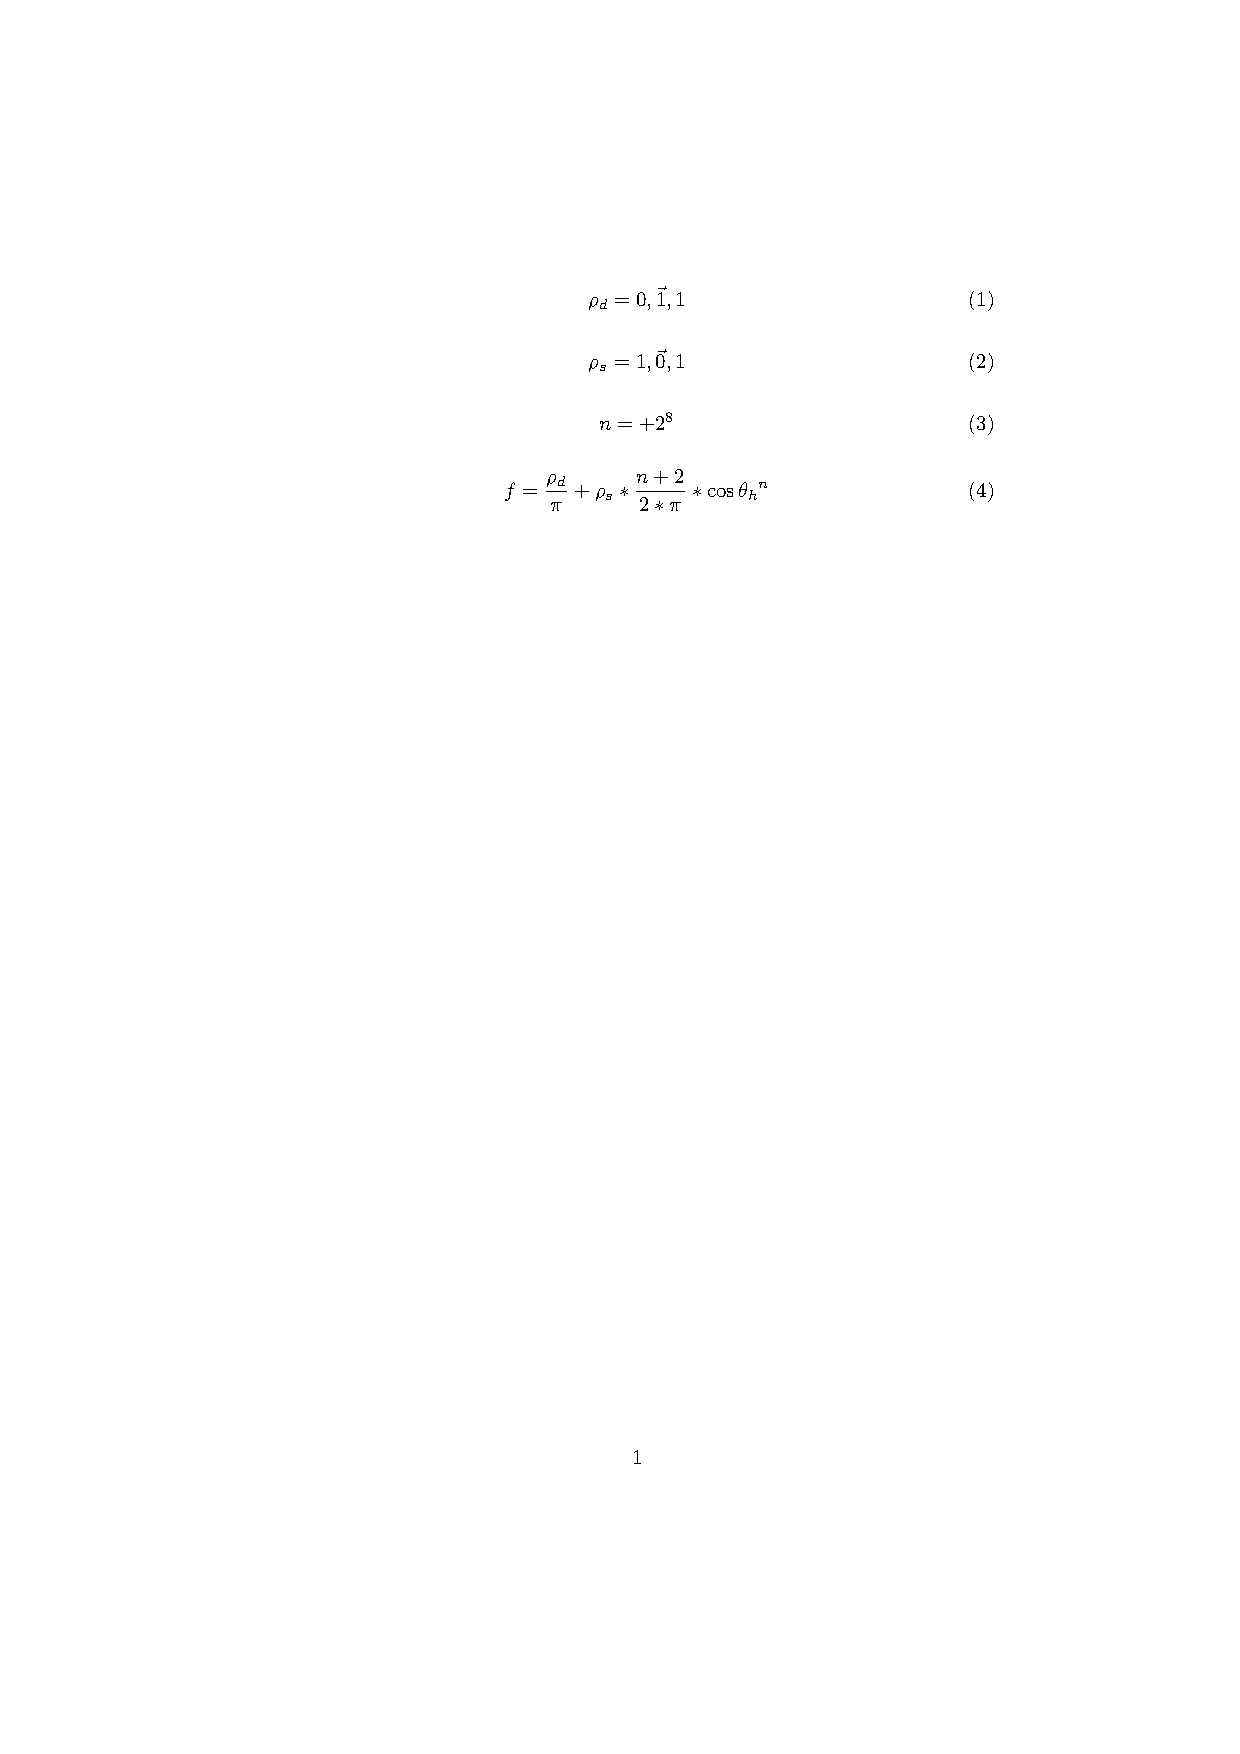
\includegraphics[scale=0.55]{./Imagens/brdfs/blinn-phong.pdf}
        \end{figure}
        
        % Coluna de figuras
        \column{0.5\textwidth}
        \vspace{-0.50cm}
        \begin{figure}[H]
            \centering
            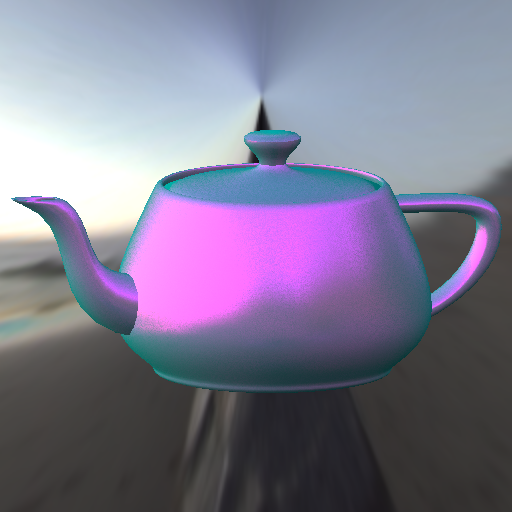
\includegraphics[height=0.32\textheight]{./Imagens/brdfs/blinn-phong-teapot.png}
            
            % {\tiny (a) \textit{Teapot}}
            
            % \vspace{0.1cm}
            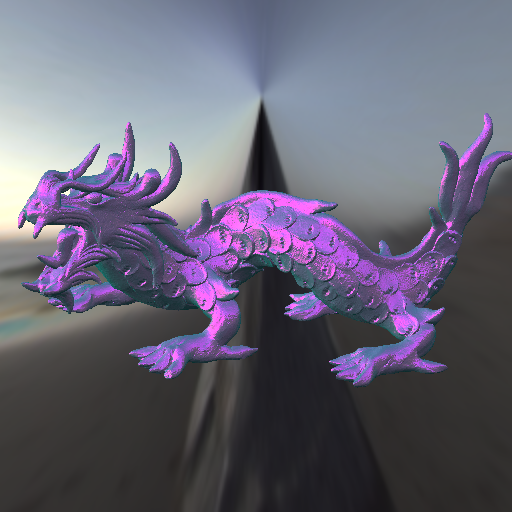
\includegraphics[height=0.32\textheight]{./Imagens/brdfs/blinn-phong-dragon.png}
            
            % \vspace{-0.5cm}
            % {\tiny (b) Dragão de Stanford}
            
            % \vspace{0.1cm}
            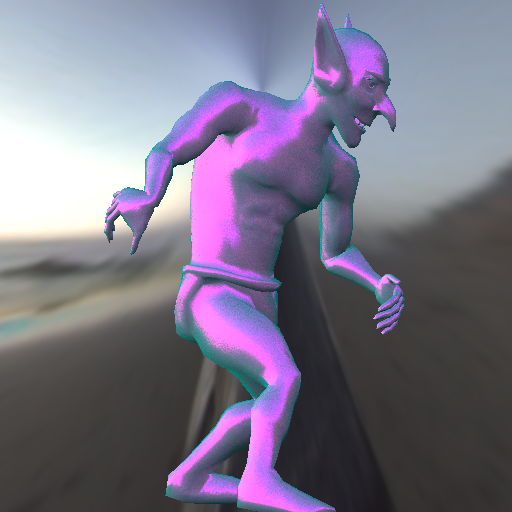
\includegraphics[height=0.32\textheight]{./Imagens/brdfs/blinn-phong-goblin.png}
            
            % \vspace{-0.4cm}
            % {\tiny (c) Goblin}
        \end{figure}
    \end{columns}
\end{frame}

\begin{frame}{Contexto - BRDF Cook-Torrance}
    \begin{columns}
        % Coluna de texto
        \column{0.5\textwidth}
        \small{}
        \vspace{-0.55cm}
        \begin{figure}
            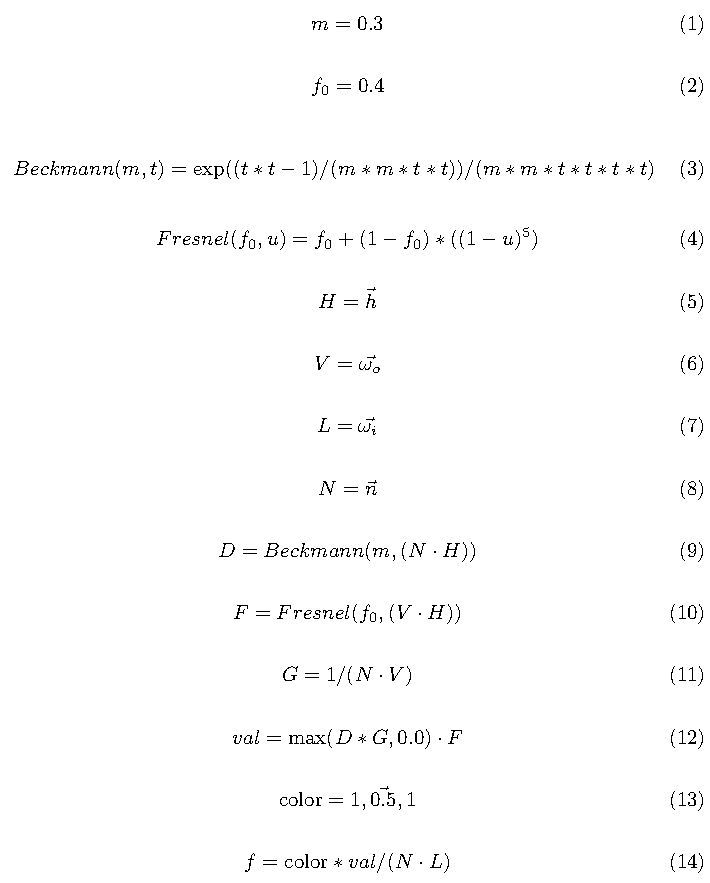
\includegraphics[scale=0.48]{./Imagens/brdfs/cook-torrance-alternative.pdf}
        \end{figure}
        
        % Coluna de figuras
        \column{0.5\textwidth}
        \vspace{-0.50cm}
        \begin{figure}[H]
            \centering
            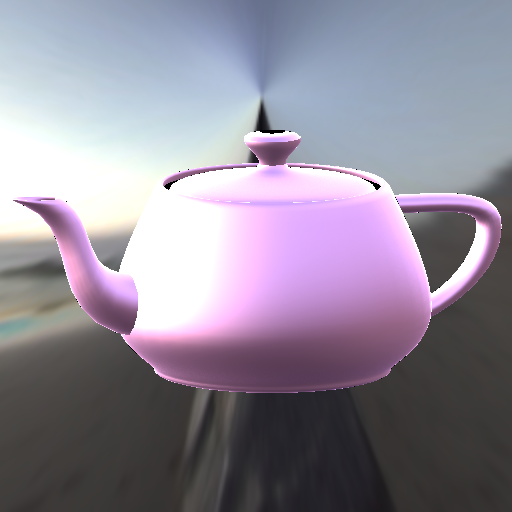
\includegraphics[height=0.32\textheight]{./Imagens/brdfs/cook-torrance-alternative-teapot.png}
            
            % {\tiny (a) \textit{Teapot}}
            
            % \vspace{0.1cm}
            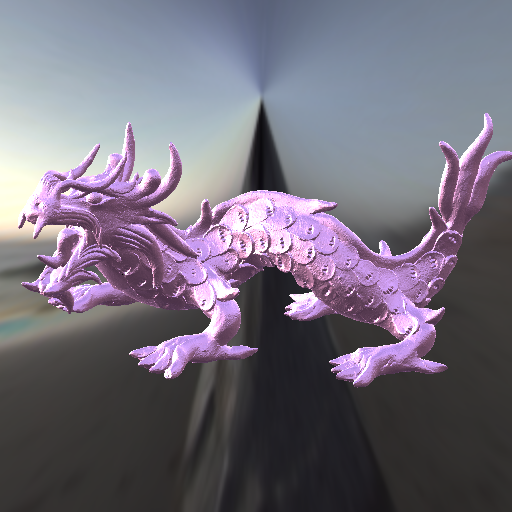
\includegraphics[height=0.32\textheight]{./Imagens/brdfs/cook-torrance-alternative-dragon.png}
            
            % \vspace{-0.5cm}
            % {\tiny (b) Dragão de Stanford}
            
            % \vspace{0.1cm}
            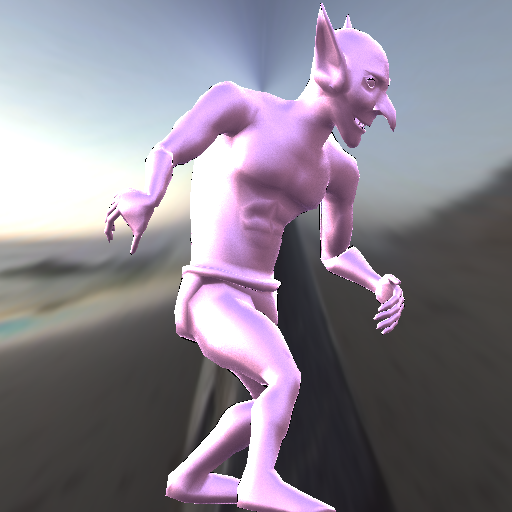
\includegraphics[height=0.32\textheight]{./Imagens/brdfs/cook-torrance-alternative-goblin.png}
            
            % \vspace{-0.4cm}
            % {\tiny (c) Goblin}
        \end{figure}
    \end{columns}
\end{frame}


\begin{frame}{Contexto - \textit{shaders}}
\begin{itemize}
\item \textit{Shaders} concedem a capacidade de cada objeto renderizado ter sua \textbf{aparência configurada por meio de um código} que implementa uma BRDF.
\end{itemize}

\end{frame}

\begin{frame}{Motivação}

    Na renderização, as BRDFs são implementadas por meio de programas chamados de \textit{\textbf{shaders}}. Mas, as BRDFs são comumente descritas por equações em \LaTeX \footnote{\tiny{ \LaTeX{} é um sistema de preparação de documentos para alta qualidade tipográfica. Assim como visto no início.}}. Dois problemas surgem com essa modelagem:

    \begin{enumerate}
        \item Barreira técnica\footnote{\tiny{Físicos ou matemático podem trabalhar com BRDFs e não, necessárimente saber programação baixo nível }}: visualizar essa modelagem de BRDFs requer conhecimento especializado em programação em linguagem de \textit{shading}.
    \item Baixo nível de iteração: toda mudança nas equações exige baixar o nível e reescrever o \textit{shader} novamente.
    \end{enumerate}

\end{frame}


\begin{frame}{Motivação}
        Surge a necessidade de \textbf{simplificar} a \textbf{criação de shaders para BRDFs}. \\\hspace{2cm}


    Um \textbf{compilador} capaz de traduzir BRDFs escritas em \LaTeX{} para \textit{shaders} permitiria uma maior acessibilidade e agilidade na criação de efeitos visuais complexos.
    \begin{figure}[H]
        \begin{center}
            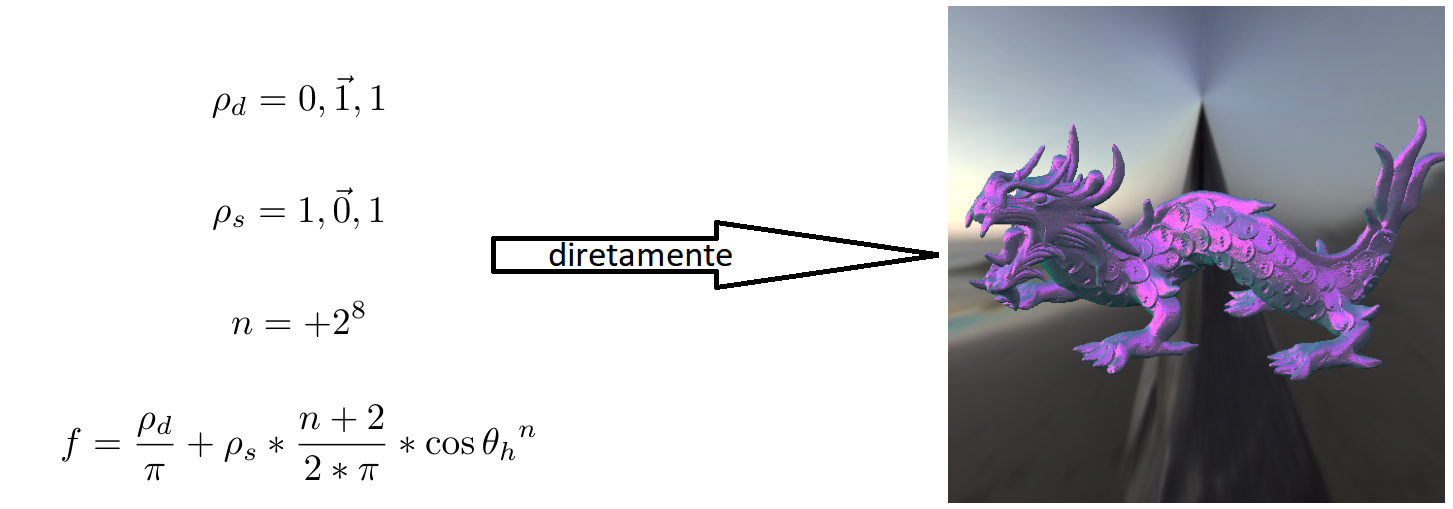
\includegraphics[width=0.65\textwidth]{./Imagens/diretamente.png}
        \end{center}
    \end{figure}
\end{frame}



\begin{frame}{Objetivo}
    Projetar e implementar um \textbf{compilador} capaz de:

    \begin{enumerate}
        \item Processar \textbf{BRDFs} descritas em equações \LaTeX{}.
        \item Gerar \textbf{código de \textit{shading}} na linguagem-alvo da API \textbf{OpenGL}.
        \item Visualizar o efeito dessas BRDFs usando o \textbf{código GLSL} gerado.
    \end{enumerate}

    Resultado esperado é um \textbf{shader} que reproduza as características de refletância da BRDF original.
\end{frame}


\section{Conceitos}

\begin{frame}{Conceitos - BRDFs}

As BRDFs calculam a proporção entre a energia luminosa que atinge um ponto na superfície e como essa energia é:
    \begin{itemize}
        \item \textbf{Refletida}
        \item \textbf{Transmitida}
        \item \textbf{Absorvida}
    \end{itemize}
    \begin{figure}[H]
        \begin{center}
            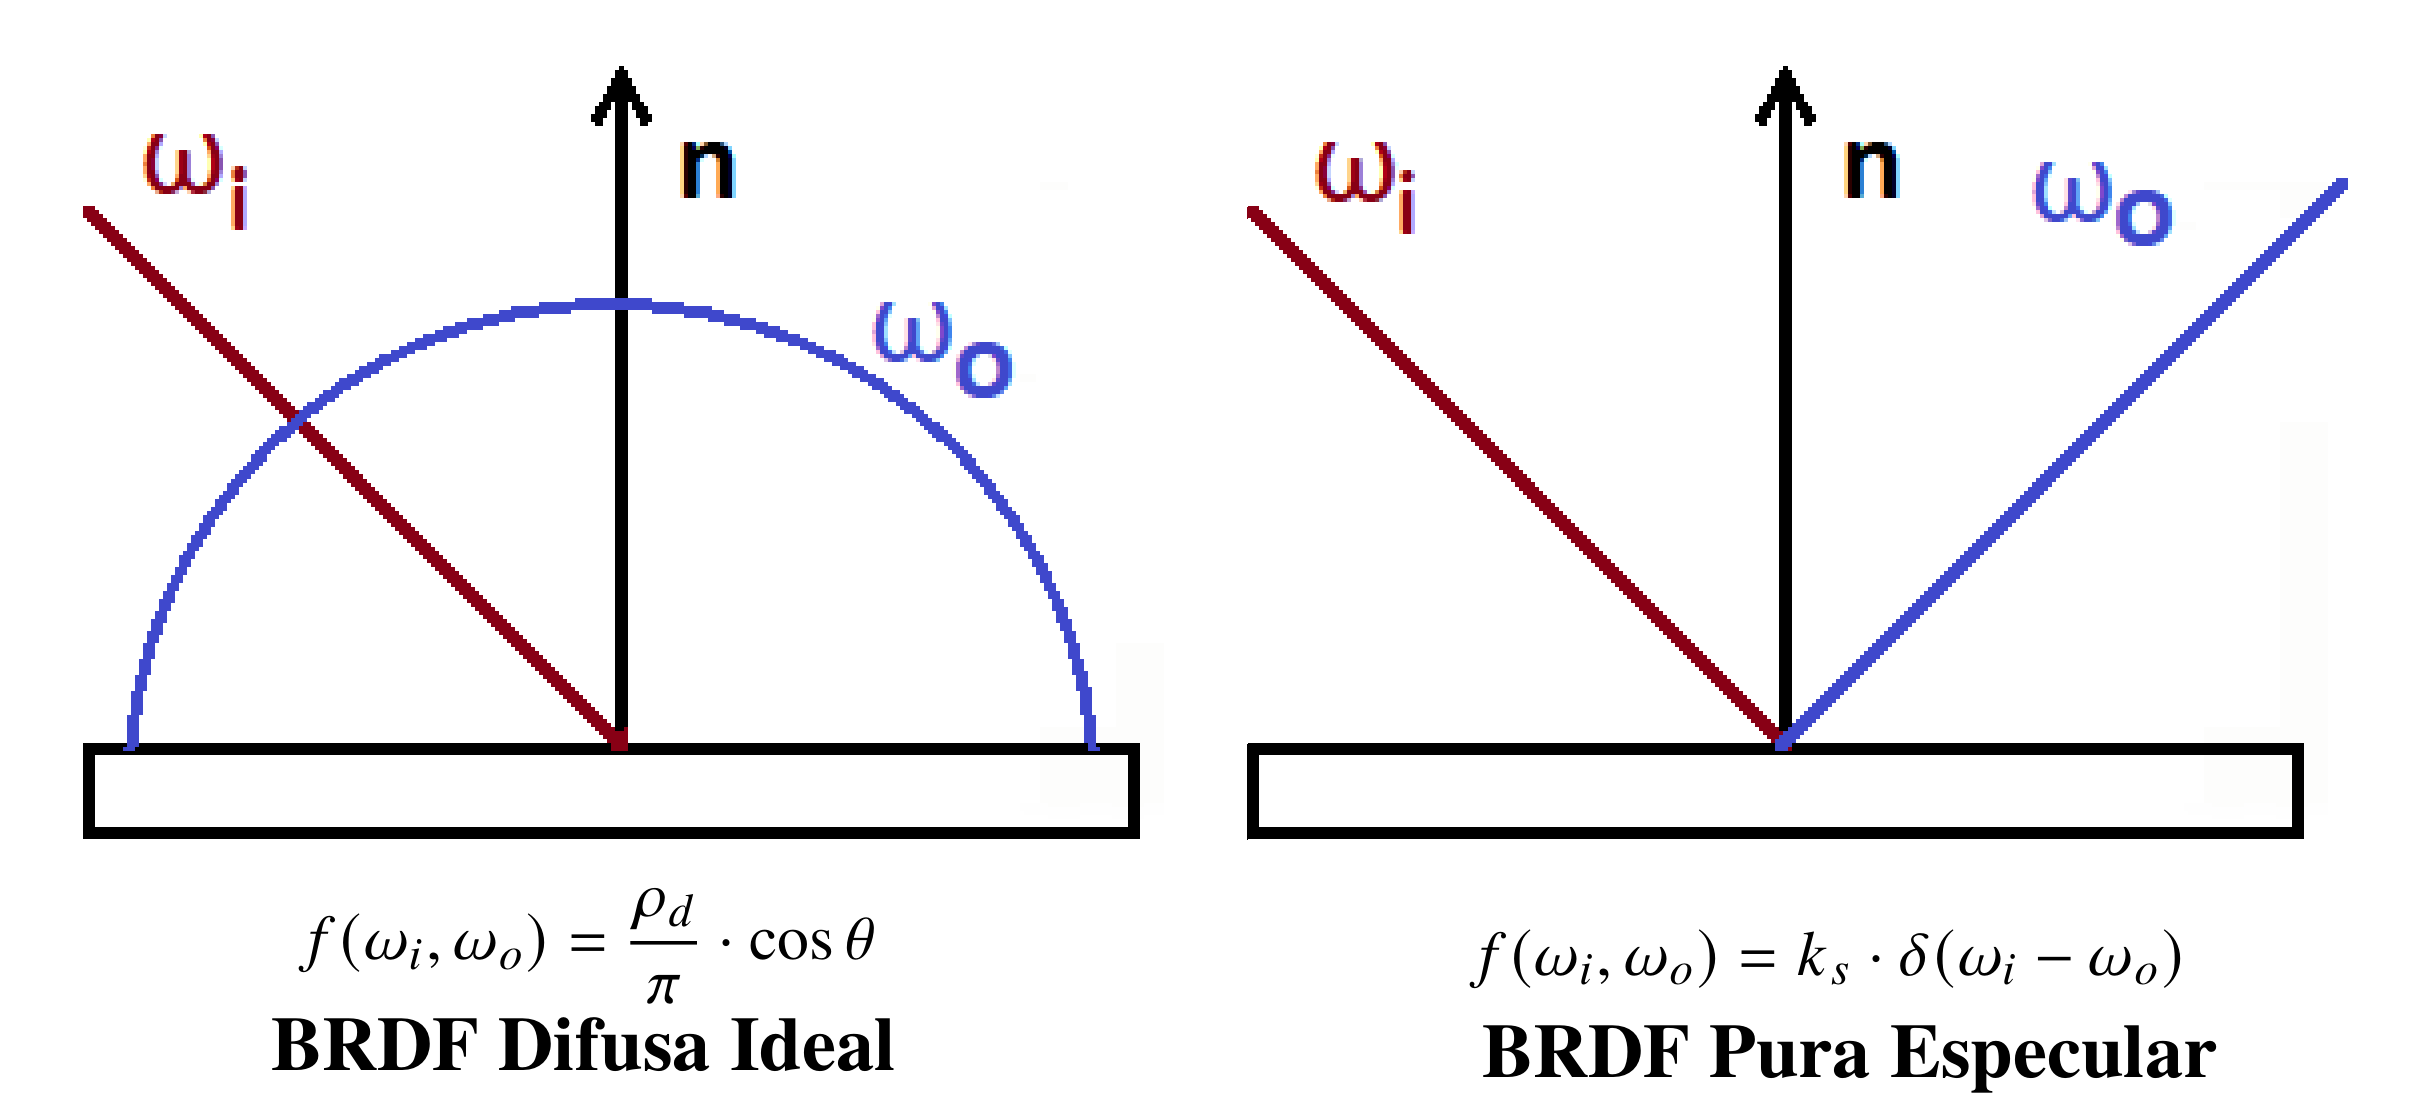
\includegraphics[width=0.65\textwidth]{./Imagens/difusa-e-specular.png}
        \end{center}
    \end{figure}
\end{frame}


\begin{frame}{Equação de Renderização}
Um renderizador estima a ``quantidade'' luz $L_o$ que sai de um ponto em uma direção ${\omega}_o$ usando a equação de renderização (\cite{rendering_equation}). Nela, a BRDF é encontrada:

    \begin{columns}
        \column{0.6\textwidth}
\begin{equation}\label{eq-rendering-equation}
\begin{aligned}
  &L_o(p, {\omega}_o) = L_e(p, {\omega}_o) +
\int_{H^2}f(p, {\omega}_i, {\omega}_o){L_i(p,{\omega}_i)\cos(\theta_i)d{\omega}_i}\\
    &L_o \text{ é radiância de saída}\\
    &L_e \text{ é radiância emitida pela superfície \tiny{(i.e. fonte de luz)}}\\
    &L_i \text{ é radiância incidente na superfície}\\
    &{\omega}_i \text{ é a direção do raio incidente}\\
    &{\omega}_o \text{ é a direção do raio refletido}\\
    % &H^2 \text{ são todas as direções no hemisfério no ponto $p$}\\
    % &\theta_i \text{ ângulo entre direção incidente e a normal da superfície}\\
    &f \text{ função de refletância}\\
\end{aligned}
\end{equation}
\column{0.4\textwidth}
    \begin{figure}[H]
        \caption{\cite{MicrofacetBRDF}}
        \vspace{2cm}
        \hspace{2cm}
        \begin{center}
            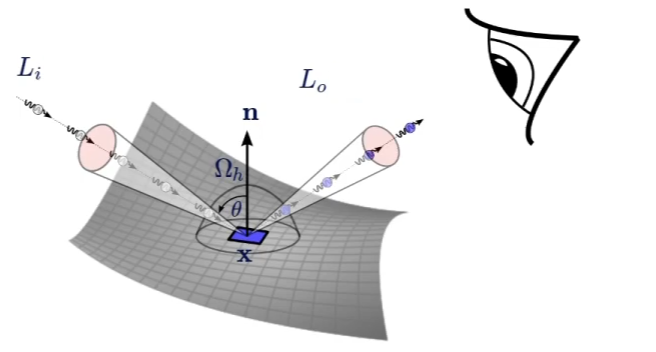
\includegraphics[width=0.65\textwidth]{./Imagens/Li-Lo.png}
        \end{center}
    \end{figure}
    \end{columns}
\end{frame}



% SLIDE 2
\begin{frame}{\textit{Pipeline} de GPU}
    Etapas Principais:
    \begin{enumerate}
        \item \textbf{\textit{Shader} de Vértice}: Processa e transforma vértices.
        \item \textbf{Rasterização}: Gera fragmentos a partir de primitivas.
        \item \textbf{\textit{Shader} de Fragmento}: Determina a cor final dos fragmentos.
    \end{enumerate}

    Fluxo de dados são:  CPU $\to$ GPU $\to$ \textit{Shaders} $\to$ Imagem final.
    \begin{figure}[H]
        % \centering
        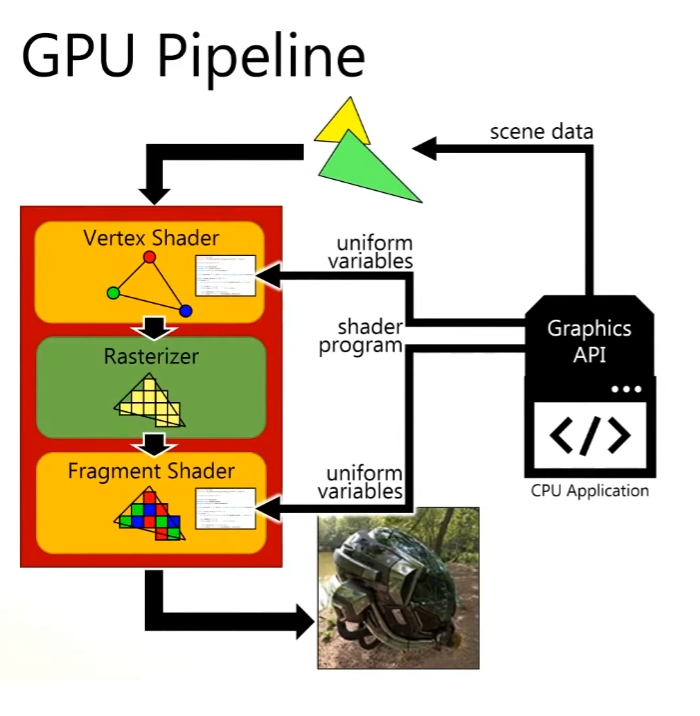
\includegraphics[scale=0.25]{./Imagens/gpu_pipeline.png}
        % \caption{\small Representação do \textit{pipeline} de GPU.}
    \end{figure}
\end{frame}

% SLIDE 3
\begin{frame}[fragile]{\textit{Shader} de Vértice}
    \begin{itemize}
        \item Aplicação de transformações (ex.: rotação, projeção).
        \item Transmissão de dados (ex.: normais) ao \textit{shader} de fragmento.
    \end{itemize}

    \begin{clang}
#version 330 core
layout(location = 0) in vec3 inPosition;
layout(location = 1) in vec3 inNormal;

uniform mat4 modelViewProjection;

out vec3 fragNormal;

void main() {
    vec3 manipulatedPosition = inPosition + (sin(gl_VertexID * 0.1) * 0.1);
    fragNormal = inNormal;
    gl_Position = modelViewProjection * vec4(manipulatedPosition, 1.0);
}
    \end{clang}
\end{frame}

% SLIDE 4
\begin{frame}{\textit{Shader} de Fragmento}
    Nesse \textit{shader} é onde a cor final é calculada. Roda paralelamente 1 vez para cada ``pixel''.
    \begin{figure}[H]
        \centering
        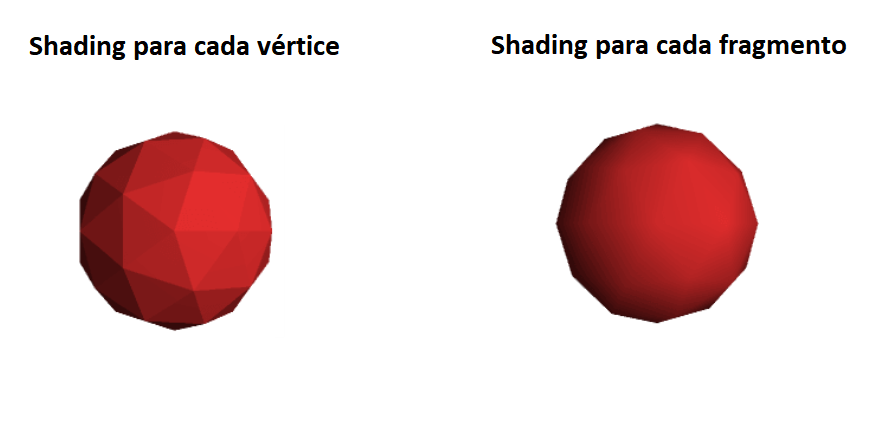
\includegraphics[scale=0.5]{./Imagens/per_vertex_per_frag.png}
        \caption{\small Diferença entre \textit{shading} por vértice e por fragmento.}
    \end{figure}
\end{frame}

% \begin{frame}{Shaders e implementação}
%     \begin{itemize}
%         \item Na renderização, BRDFs são implementadas por \textit{shaders}, programas especializados executados na GPU.
%         \item APIs gráficas permitem programar esses shaders em diferentes etapas do processo de renderização ( OpenGL).
%         \item Com os shaders, cada objeto renderizado pode ter sua aparência configurada por meio de códigos que implementam BRDFs específicas.
%     \end{itemize}
% \end{frame}

\begin{frame}{Compilação: Visão Geral}
    Compilador $C: L_1 \rightarrow L_2$ mapeia programa de $L_1$ para $L_2$ preservando semântica\footnote{\tiny{Mantém mesmo significado algorítmico}}.

    \begin{enumerate}

        \item \textbf{Análise Léxica (Lexing):}
              \begin{itemize}
                  \item Divide entrada em tokens (palavras-chave, identificadores)
                  \item Reconhecível por máquinas de estado
              \end{itemize}
        \item \textbf{Análise Sintática (Parsing):}
              \begin{itemize}
                  \item Constrói árvore sintática baseado nas regras de produção
              \end{itemize}
        \item \textbf{Verificação Semântica:}
              \begin{itemize}
                  \item Garante consistência de tipos, assinatura de funções, significado dos símbolos, etc.
                  \item No nosso caso, previne erros na modelagem da BRDF
              \end{itemize}
        \item \textbf{Emissão de Código:}
              \begin{itemize}
                  \item Gera código na linguagem alvo
              \end{itemize}
    \end{enumerate}
\end{frame}


\section{Metodologia}

\begin{frame}{Metodologia: Análise e Técnicas}
      \textbf{Estudo da Literatura:}
             \begin{itemize}
                 \item Nenhum trabalho similar encontrado em bases acadêmicas
             \end{itemize}

\begin{table}[H]
\scriptsize
  \caption{\tiny Resultados das bases após aplicar os critérios.}
\label{tab-result}
\begin{tabular}{l|c}
\scriptsize
  %\hline
   \textbf{Bases}  & \textbf{Filtrados}\\
   \hline
    IEEE Xplore Digital Library
    % NOTE: Eram 2, mas removi 'Tree-Structured Shading Decomposition'.
    % NOTE: Decidi voltar para 2 e incluir novamente o artigo removido
   & 2
    \\ \hline
    BDTD
    & 0
    \\ \hline
    CAPES Periódico
    & 0
    \\ \hline


  ACM Digital Library
  & 1
    \\ \hline
 Google Acadêmico
  & 1
   % \hline
\end{tabular}
\end{table}
       
      \textbf{Estudo Realizado} nas seguintes áreas:
             \begin{itemize}
                 \item Radiometria e BRDFs. Base teórica pelo livro ''Physically Based Rendering`` \cite{pbr}.
                 \item Linguagem de shader GLSL
                 \item Técnicas de análise sintática (Pratt Parsing) e geração de código
                 \item Análise de BRDFs existentes (Artigos)
             \end{itemize}

\end{frame}

\begin{frame}[fragile]{Metodologia: Design Inicial de Casos de Teste}
    Design inicial para validação da tradução BRDF em \LaTeX{} $\to$ GLSL\footnote{\tiny{Alguns símbolos não estão definidos para simplificar}}

   { \small
   \begin{equation*}
       \text{cook\_torrance}(\omega_i, \omega_o) = \frac{D(h)F(\omega_i, h)G(\omega_i, \omega_o, h)}{4(\omega_i \cdot n)(\omega_o \cdot n)}
   \end{equation*}
   }

    \vspace{1cm}
   \begin{columns}
       
       % Coluna do código LaTeX
       \column{0.5\textwidth}
       \LaTeX{} Fonte
       \begin{lstlisting}[basicstyle=\scriptsize]
\text{cook\_torrance}(\omega_i, \omega_o)
   = \frac{D(h)F(\omega_i, h)G(\omega_i,
   \omega_o, h)}{4(\omega_i \cdot n)
   (\omega_o \cdot n)}
       \end{lstlisting}
       
       % Coluna do GLSL
       \column{0.5\textwidth}
       GLSL a ser gerado
       \begin{lstlisting}[language=C, basicstyle=\tiny]
vec3 cook_torrance(vec3 wi, vec3 wo) {
   float D_RESULT = D(h);
   vec3  F_RESULT = F(wi, wo);
   float G_RESULT = G(wi, wo, h);
   float den = 4.0 * dot(n, wi) * dot(n, wo);
   return D_RESULT * F_RESULT * G_RESULT / den;
}
       \end{lstlisting}
   \end{columns}
   
   % \vspace{0.3cm}

\end{frame}

\begin{frame}{Metodologia: Implementação do Compilador}
   \begin{columns}
       % Coluna de texto principal
       \column{0.65\textwidth}
       \begin{itemize}
           \item \textbf{Linguagem Odin:}
                 \begin{itemize}
                     \item Linguagem de propósito geral, orientada a dados
                     \item Sem dependências externas (biliotecas padrão)
                 \end{itemize}
           \item \textbf{Etapas do Compilador:}
                 \begin{itemize}
                     \item Lexer e Parser (Pratt Parsing)
                     \item Análise Semântica (checker)
                     \item Travessia AST (walker)
                     \item Geração GLSL (emitter)
                 \end{itemize}
       \end{itemize}
       
       % Coluna da direita com diagrama simples
       \column{0.35\textwidth}
       \begin{tikzpicture}[node distance=1.2cm]
           \node[draw] (latex) {LaTeX};
           \node[draw, below of=latex] (lexer) {Lexer};
           \node[draw, below of=lexer] (parser) {Parser};
           \node[draw, below of=parser] (checker) {Checker};
           \node[draw, below of=checker] (emitter) {Emitter};
           \node[draw, below of=emitter] (glsl) {GLSL};
           
           \draw[->] (latex) -- (lexer);
           \draw[->] (lexer) -- (parser);
           \draw[->] (parser) -- (checker);
           \draw[->] (checker) -- (emitter);
           \draw[->] (emitter) -- (glsl);
       \end{tikzpicture}
   \end{columns}
\end{frame}

\begin{frame}[fragile]{Metodologia: Especificação da Linguagem}
    Subconjunto do ambiente equation (\verb|\begin{equation}|) essencial para descrever BRDFs
\begin{table}
\centering
    \scriptsize % or \footnotesize or \scriptsize
\begin{tabular}{l|l|l}
% \begin{tabularx}{\textwidth}{|L|L|L|}
\hline
    \textbf{Descrição} & \textbf{Exemplos} & \textbf{Comando \LaTeX{}} \\ \hline

    Funções trigonométricas & $\tan, \sin, \cos$ {\tiny e suas funções inversas}
    &\small\verb"\tan", \verb"\sin", \verb"\cos"
    \newline\verb"\arctan", \verb"\arcsin", $\dots$
    \\ \hline
    Função raiz quadrada & $\sqrt{}$ & \verb|\sqrt| \\ \hline
    Função exponencial & $\exp{}$ & \verb|\exp| \\ \hline
    Funções utilitárias & $\max, \min$ & \verb|\max, \min| \\ \hline
    Definições de equações & $f = x$ & \verb|f = x| \\ \hline
    Definições de funções & $f(x, y) = x^y$ & \verb|f(x, y) = x^y| \\ \hline
    Constantes comuns & $\pi$, $\epsilon$ & \verb|\pi, \epsilon| \\ \hline
    Constantes de radiometria & $\theta_i$ {\tiny e outras presentes na \autoref{tab-conventions-metodologia}} & \verb|\theta_i| \\ \hline
    Indicadores de vetor & $\vec{n}$ & \verb|\vec{}| \\ \hline
    Identificadores aninhados & $f_{n_{i}}$ & \verb|f_{n_{i}}| \\ \hline
    Chamadas de funções & $f(x + y)$ & \verb|f(x + y)| \\ \hline
    Produto vetorial & $x \times y$ & \verb|x \times y| \\ \hline
    Soma e Subtração & $x + y$, $x - y$ & \verb|x + y|, \verb|x - y| \\ \hline
    Negação & $-y$ & \verb|-y| \\ \hline
    Multiplicação & $x \cdot y$ & \verb|x \cdot y| \\ \hline
    Frações & $\frac{x}{y}$ & \verb|\frac{x}{y}| \\ \hline
    Divisão & $x / y$ & \verb|x / y| \\ \hline
    Potenciação & $x^y$ & \verb|x^y| \\ \hline
\end{tabular}
\caption{Tabela de especificação da linguagem.}
\label{tab-definition-of-lang}
\end{table}
\end{frame}


\begin{frame}[fragile]{Metodologia: Especificação de Convenções}
    Convenções sobre BRDFs suportadas
\begin{table}
\centering
    \scriptsize % or \footnotesize or \scriptsize
\begin{tabular}{l|l|l}
        \hline
        \textbf{Símbolo} &\textbf{Comando \LaTeX{}} & \textbf{Descrição} \\
        \hline
         $\theta_i$ & \verb"\theta_i" &Ângulo de elevação da direção da luz incidente \\ \hline
         $\theta_o$ & \verb"\theta_o" &Ângulo de elevação da direção da luz refletida \\ \hline
         $\phi_i$   & \verb"\phi_i"   &Ângulo azimutal da direção da luz incidente \\ \hline
         $\phi_o$   & \verb"\phi_o"   &Ângulo azimutal da direção da luz refletida \\ \hline
         $\omega_i$ & \verb"\omega_i" &Direção da luz incidente  \\ \hline
         $\omega_o$ & \verb"\omega_o" &Direção da luz refletida  \\ \hline
         $f$        & \verb"f"        &BRDF de referência \\ \hline
         $\vec{n}$  & \verb"\vec"     &Vetor normal à superfície \\ \hline
         $\vec{h}$  & \verb"\vec"     &Vetor do meio entre $\omega_o$ e $\omega_i$ \\ \hline
         $\theta_h$ & \verb"\theta_h" &Ângulo entre $\vec{n}$ e $\vec{h}$ \\ \hline
         $\theta_d$ & \verb"\theta_d" &Ângulo entre $\omega_i$ e $\vec{h}$ \\ \hline
\end{tabular}
    \caption{Tabela de símbolos e suas descrições}
    \label{tab-conventions-metodologia}
\label{tab-definition-of-lang}
\end{table}
\end{frame}

\begin{frame}[fragile]{Metodologia: Experimentos de Renderização}
   \begin{columns}
       % Coluna de texto
       \column{0.45\textwidth}
       Escolha da ferramenta: \textbf{Disney BRDF Explorer:}
             \begin{itemize}
                 \item Aceita shaders para renderizador em tempo real
                 \item Interface interativa
                 \item Ajuste dinâmico de parâmetros
             \end{itemize}
       % Coluna direita: imagem e código
       \column{0.55\textwidth}
       \begin{figure}
           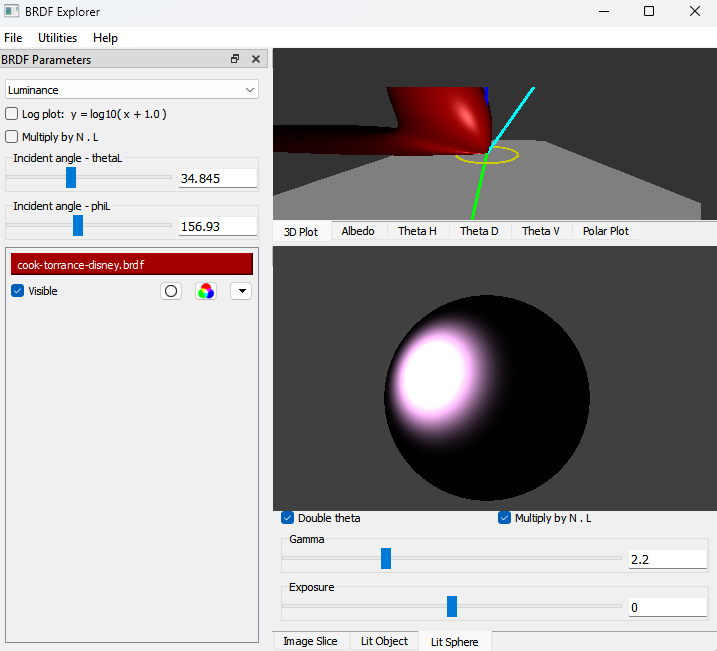
\includegraphics[width=0.65\textwidth]{./Imagens/disney-brdf-tool-original2.png}
           % \caption{\small Interface do Disney BRDF Explorer}
       \end{figure}

% \begin{lstlisting}[basicstyle=\tiny,language=C]
% ::begin parameters
% float n 1 1000 100
% ::end parameters
% ::begin shader
% vec3 BRDF(...) {
%    // código gerado
% }
% ::end shader
% \end{lstlisting}
    \end{columns}
\end{frame}

\section{Desenvolvimento}

% Slide 2: Estrutura de Pacotes
\begin{frame}{Desenvolvimento - Arquitetura do Compilador}
    \begin{itemize}
        \item Organização modular para encapsulamento de responsabilidades:
        \begin{itemize}
            \item \texttt{lexer}: Análise léxica e tokenização.
            \item \texttt{parser}: Construção da AST com \textit{Pratt Parsing}.
            \item \texttt{walker}: Navegação e análise da AST.
            \item \texttt{checker}: Inferência de tipos e validações semânticas.
            \item \texttt{emitter}: Geração do código GLSL.
        \end{itemize}
    \end{itemize}
    \begin{figure}
        \centering
        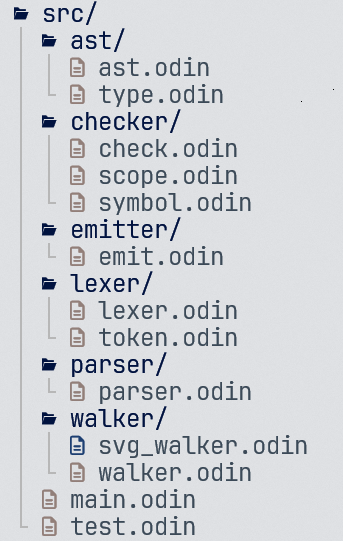
\includegraphics[scale=0.34]{./Imagens/package-structure.png}
        \caption{\small Estrutura de pacotes do compilador.}
    \end{figure}
\end{frame}


\begin{frame}{Arquitetura do Compilador}
    \begin{figure}
        \centering
        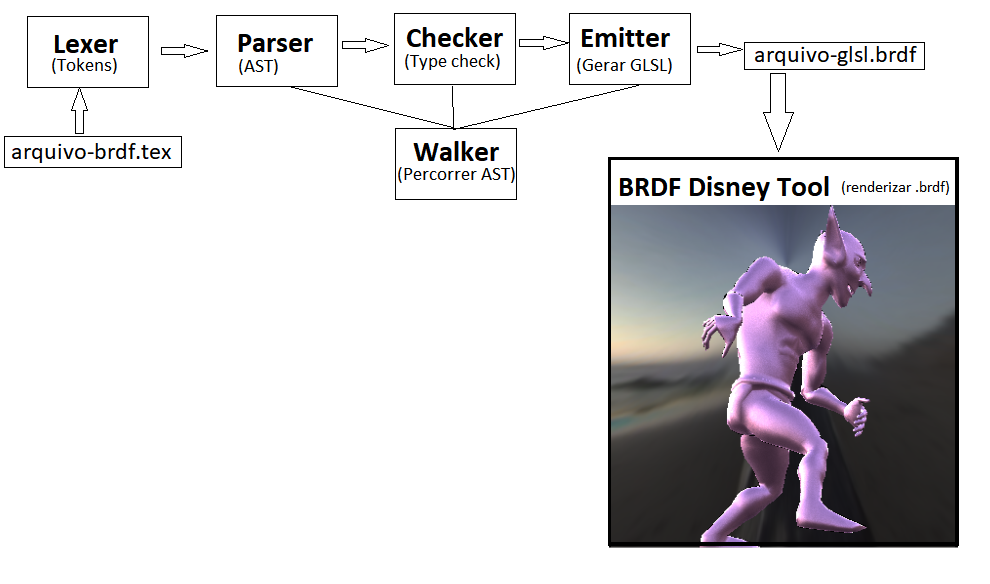
\includegraphics[scale=0.35]{./Imagens/estutura-geral-do-projeto.png}
        \caption{\small Estrutura geral da arquitetura do compilador.}
    \end{figure}
\end{frame}

\begin{frame}{Destaques do Desenvolvimento}
    \begin{itemize}
        \item Análise sintática baseada em \textit{Pratt Parsing}, garantindo precisão e hierarquia nas expressões.
        \item Funcionalidades do \texttt{walker}:
        \begin{itemize}
            \item Navegação genérica e preparação para verificações.
            \item Suporte uniforme à travessia de nós.
        \end{itemize}
        \item Integração do \texttt{checker} com a tabela de símbolos para validações semânticas e consistência.
        \item Geração de \textit{shaders} GLSL compatíveis com Disney BRDF Explorer.
    \end{itemize}
\end{frame}


\section{Resultados}

\begin{frame}{Resultados}
    Experimentos são relizados com diferentes BRDFs para validar o compilador
   \begin{itemize}
       \item Metodologia padronizada:
             \begin{itemize}
                 \item O código fonte de entrada são equações no ambiente \texttt{equation} do \LaTeX{}
                 \item Tradução para GLSL pelo compilador desenvolvido neste trabalho
                 \item Visualização no Disney BRDF Explorer
             \end{itemize}
       \item Condições controladas:
             \begin{itemize}
                 \item Ângulos de luz fixos ($\theta_i = 33.89°$, $\phi_i = 145.83°$)
                 \item Gamma = 2.112, Exposição = -1.248
             \end{itemize}
   \end{itemize}
\end{frame}

\begin{frame}{Resultados: Experimentos}

\begin{itemize}
\item \textbf{11 Experimentos Realizados:}
    \begin{enumerate}
        \item Blinn-Phong
        \item Cook-Torrance
        \item Ward 
        \item Ashikhmin-Shirley
        \item Oren-Nayar 
        \item Cook-Torrance$_2$
        \item Ashikhmin-Shirley$_2$ 
        \item Dür
        \item Edwards-2006
        \item Kajiya-Kay-1989$_*$
        \item Minnaert
    \end{enumerate}
         % \begin{enum}
         %     \item Modelos Comuns:
         %     \item Modelos Avançados:
         %     \item Variações:
         %     \item Especializados/Outros:
         % \end{itemize}

\item Cada experimento ilustra:
         \begin{enumerate}
             \item Código fonte de entrada (\LaTeX{}) e saída (GLSL)
             \item Gráficos 3D e 2D de distribuição de reflexão
             \item Renderização de objetos 3D
         \end{enumerate}

    \end{itemize}
\end{frame}


%%%%%%%%%%%%%%%%%%%%%%%%%%%%%%%%%%%%%%%%%%%%%%%%%
% \subsection{Experimento Blinn-Phong}
%%%%%%%%%%%%%%%%%%%%%%%%%%%%%%%%%%%%%%%%%%%%%%%%%

\begin{frame}
\begin{figure}
    \frametitle{Experimento Blinn-Phong: Equações da BRDF em documento \LaTeX{}}
    \begin{center}
        % 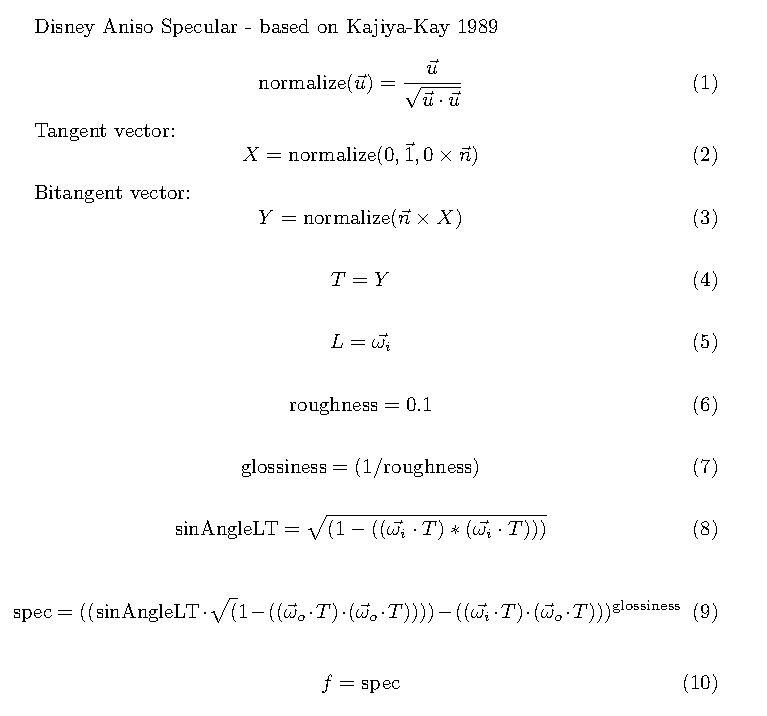
\includegraphics[scale=1.1,width=\textwidth]{./Imagens/brdfs/aniso.pdf}
        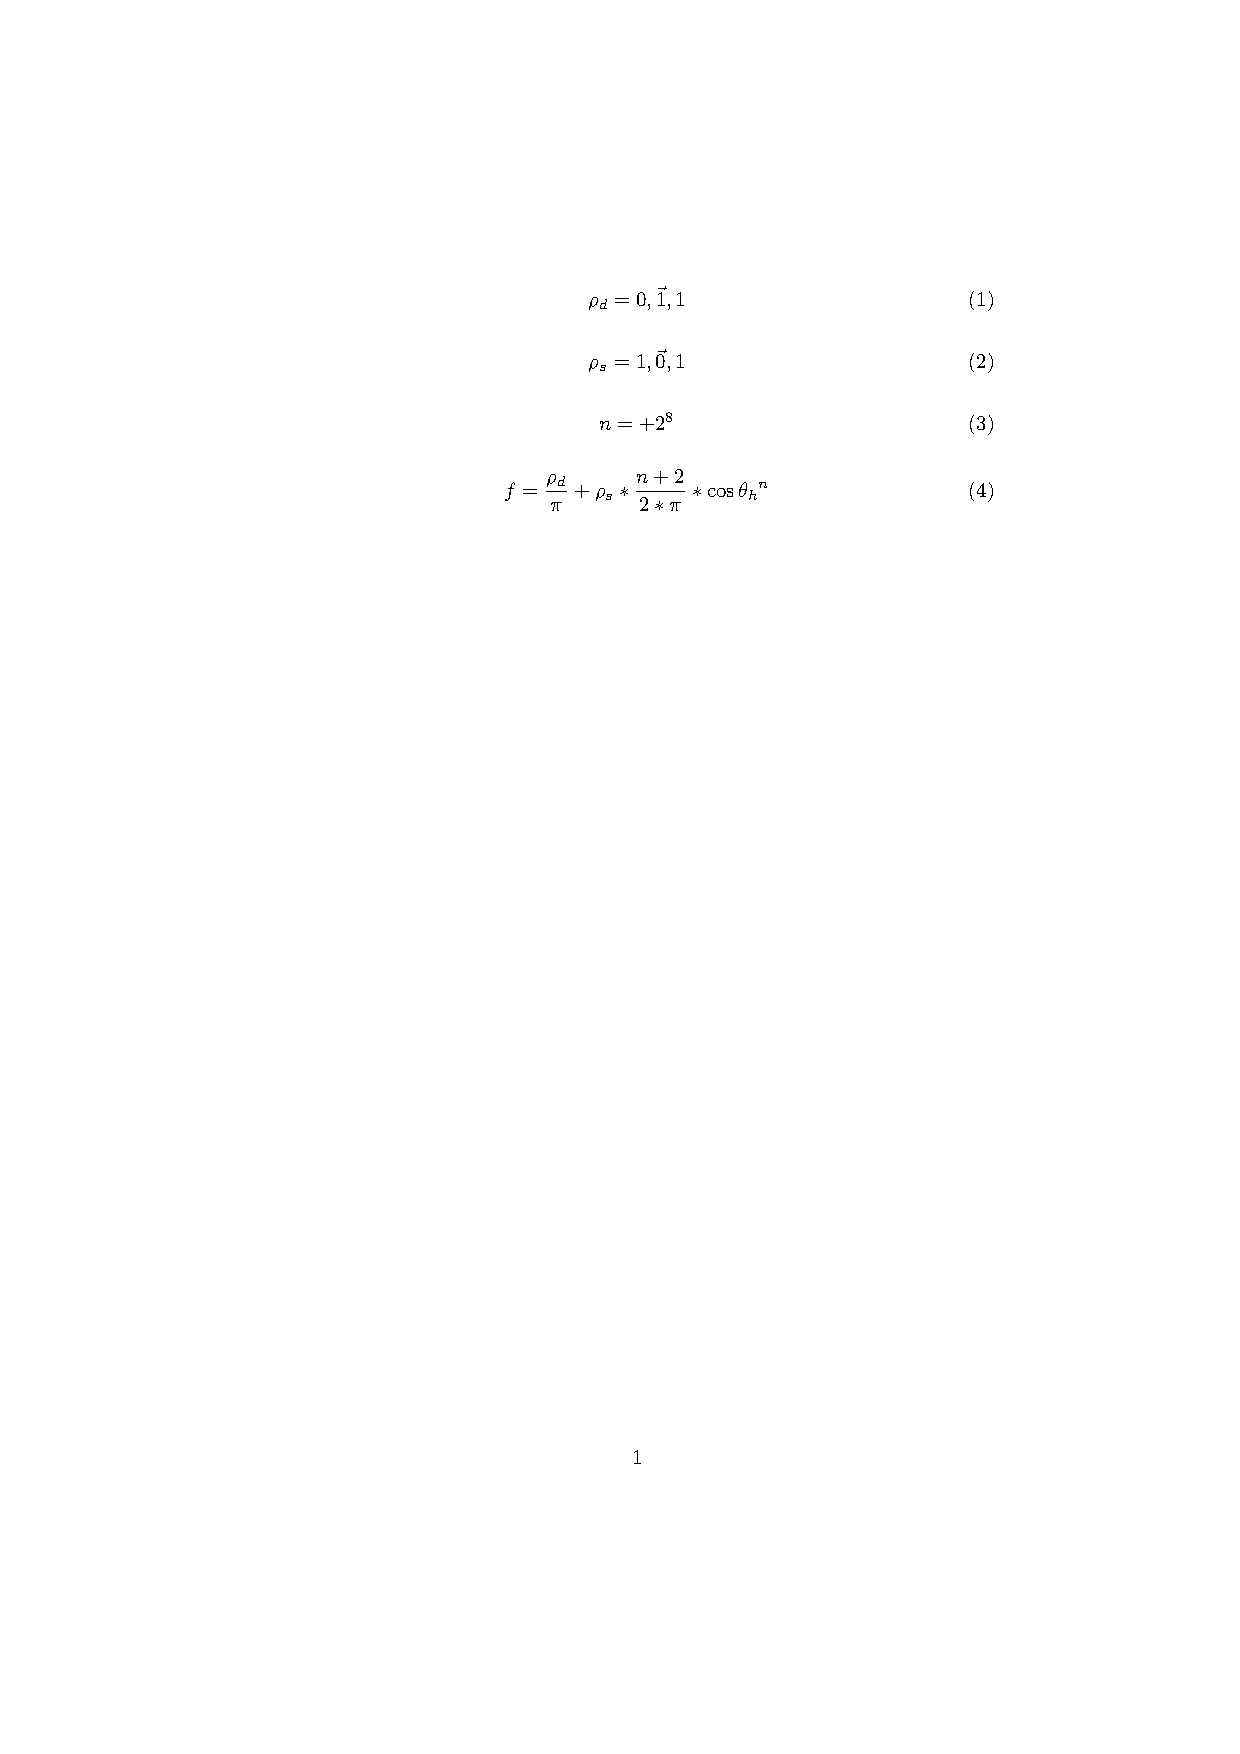
\includegraphics[scale=0.92]{./Imagens/brdfs/blinn-phong.pdf}
    \end{center}
\end{figure}
\end{frame}

%%%%%%%%%%%%%%%%%%%%%%%%%%%%%%%%%%%%%%%%%%%%%%%%%
\begin{frame}[fragile]
    \frametitle{Experimento Blinn-Phong: Código fonte \LaTeX{} da BRDF}
%%%%%%%%%%%%%%%%%%%%%%%%%%%%%%%%%%%%%%%%%%%%%%%%%
\begin{lstlisting}[language=tex, frame=none, inputencoding=utf8]
\begin{equation}
    \rho_{d} = \vec{0,1,1}
\end{equation}

\begin{equation}
    \rho_{s} = \vec{1,0,1}
\end{equation}

\begin{equation}
    n = +2^8
\end{equation}

\begin{equation}
f = \frac{\rho_{d}}{\pi} + \rho_{s} * \frac{n+2}{2*\pi} *
\cos{\theta_{h}}^{n}
\end{equation}
\end{lstlisting}
\end{frame}

\begin{frame}[fragile]
    \frametitle{Experimento Blinn-Phong: Código GLSL da BRDF deste experimento (1 de 2)}
\begin{clang}
analytic ::begin parameters
#[type][name][min val][max val][default val]
::end parameters
::begin shader
//////////// START OF BUILTINS DECLARTION ////////////
vec3 var_0_vec_h;
vec3 var_3_vec_n;
float var_10_theta_h;
float var_11_theta_d;
float var_1_pi;
float var_2_epsilon;
vec3 var_4_vec_omega_i;
float var_5_theta_i;
float var_6_phi_i;
vec3 var_7_vec_omega_o;
float var_8_theta_o;
float var_9_phi_o;
//////////// END OF BUILTINS DECLARTION ////////////
//////////// START OF USER DECLARED ////////////
vec3 var_12_rho_s;
float var_13_n;
vec3 var_14_rho_d;
vec3 var_15_f;
//////////// END OF USER DECLARED ////////////
\end{clang}
\end{frame}

\begin{frame}[fragile]
    \frametitle{Experimento Blinn-Phong: Código GLSL da BRDF deste experimento (2 de 2)}
\begin{clang}
vec3 BRDF(vec3 L, vec3 V, vec3 N, vec3 X, vec3 Y) {
  //////////// START OF BUILTINS INITIALIZATION ////////////
  var_0_vec_h = normalize(L + V);
  var_3_vec_n = normalize(N);
  var_1_pi = 3.141592653589793;
  var_2_epsilon = 1.192092896e-07;
  var_4_vec_omega_i = L;
  var_5_theta_i = atan(var_4_vec_omega_i.y, var_4_vec_omega_i.x);
  var_6_phi_i = atan(sqrt(var_4_vec_omega_i.y * var_4_vec_omega_i.y +
                          var_4_vec_omega_i.x * var_4_vec_omega_i.x),
                     var_4_vec_omega_i.z);
  var_7_vec_omega_o = V;
  var_8_theta_o = atan(var_7_vec_omega_o.y, var_7_vec_omega_o.x);
  var_9_phi_o = atan(sqrt(var_7_vec_omega_o.y * var_7_vec_omega_o.y +
                          var_7_vec_omega_o.x * var_7_vec_omega_o.x),
                     var_7_vec_omega_o.z);
  var_10_theta_h = acos(dot(var_0_vec_h, N));
  var_11_theta_d = acos(dot(var_0_vec_h, var_4_vec_omega_i));
  //////////// END OF BUILTINS INITIALIZATION ////////////
  var_12_rho_s = vec3(1.0, 0.0, 1.0);
  var_13_n = pow(2.0, 8.0);
  var_14_rho_d = vec3(0.0, 1.0, 1.0);
  var_15_f = ((var_14_rho_d / var_1_pi) +
              ((var_12_rho_s * ((var_13_n + 2.0) / (2.0 * var_1_pi))) *
               pow(cos(var_10_theta_h), var_13_n)));
  return vec3(var_15_f);
}
\end{clang}
\end{frame}

\begin{frame}{Experimento Blinn-Phong: Plots de Distruição de Reflexão}
\begin{figure}[H]
  
\caption{\small{\textit{Plots} da distribuição de reflexão especular e difusa do experimento Blinn-Phong.}}
    \label{fig-blinn-phong-plots}
\minipage{0.48\textwidth}
    \vspace{42px}
  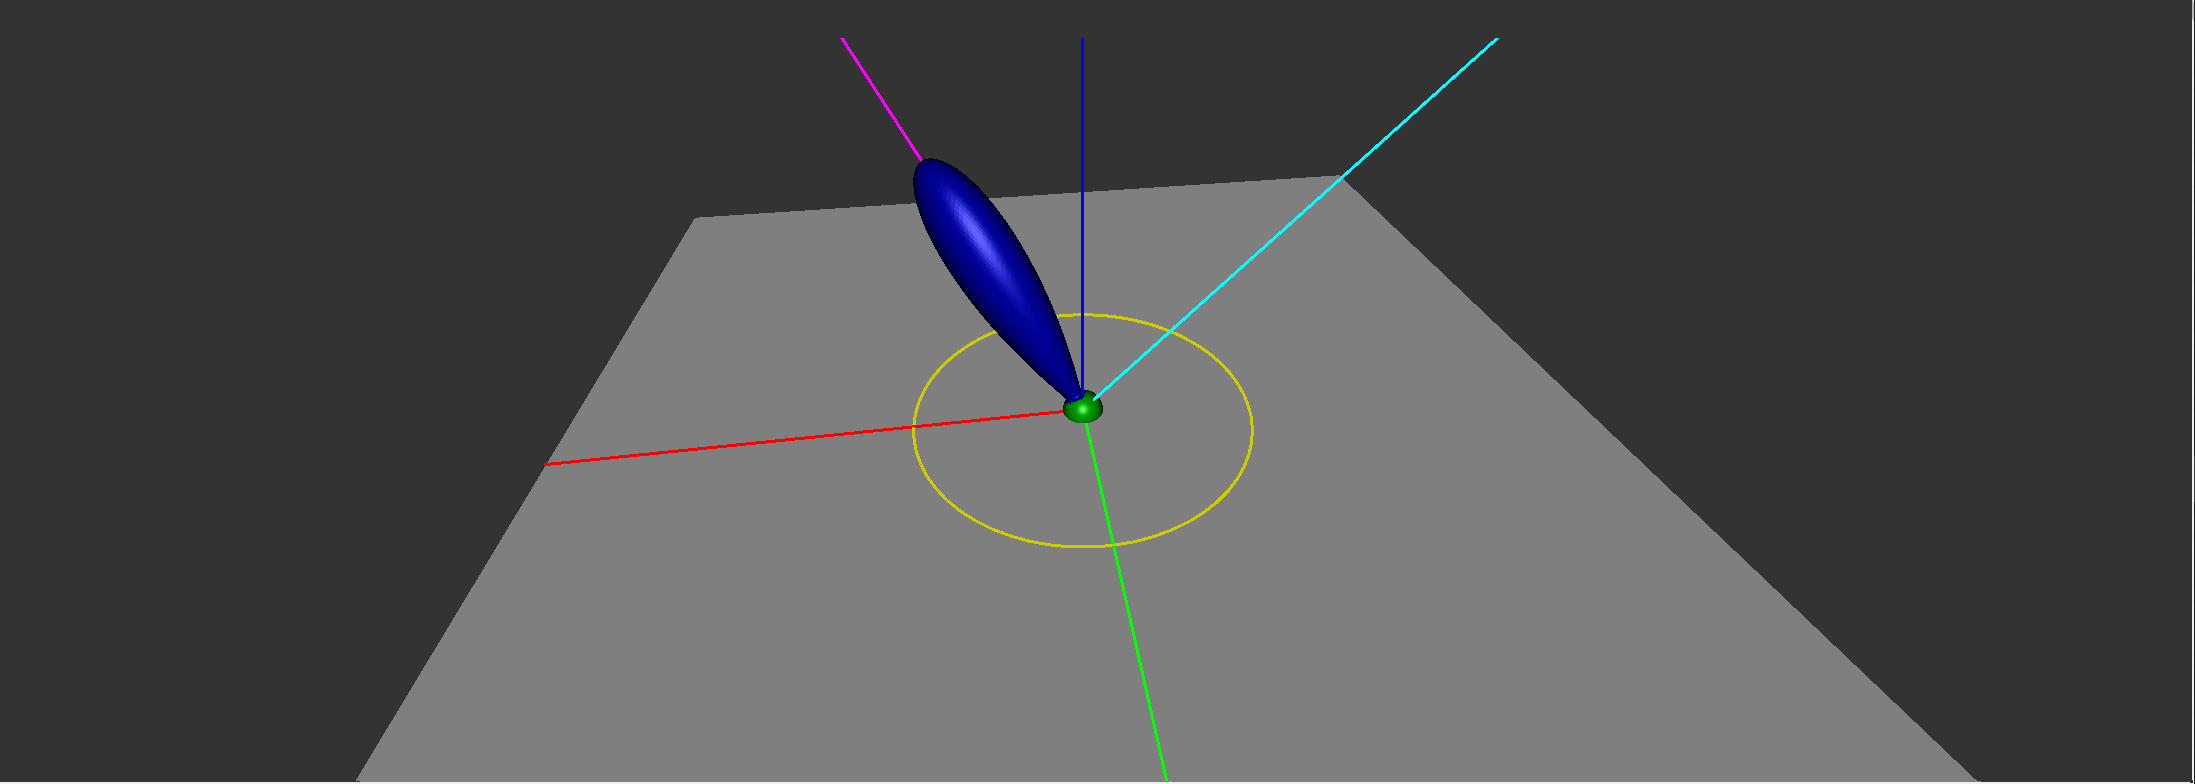
\includegraphics[width=\linewidth]{./Imagens/brdfs/blinn-phong-3D-plot}
    % \caption{\small{(a)}}\label{fig:awesome_image1}
    % \vspace{0.1px}
    % \legend{ \small (a) 3D \textit{plot}}
\endminipage\hfill
\minipage{0.48\textwidth}
  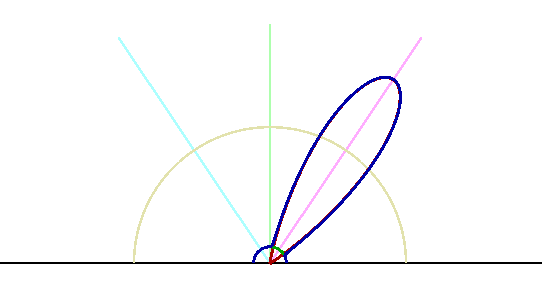
\includegraphics[width=\linewidth]{./Imagens/brdfs/blinn-phong-polar-plot-log.png}
    % \legend{ \small (b) \textit{Polar plot}}
    % \caption{\small{(b)}}\label{fig:awesome_image1}
\endminipage\hfill
\end{figure}
\end{frame}

\begin{frame}{Experimento Blinn-Phong: Objetos 3D renderizados para esta BRDF.}
\begin{figure}[H]
    \label{fig-blinn-phong-eqlang}
\minipage{0.32\textwidth}
  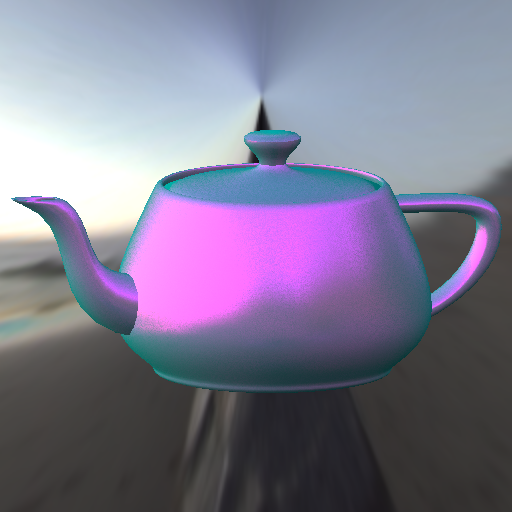
\includegraphics[width=\linewidth]{./Imagens/brdfs/blinn-phong-teapot.png}
    % \legend{ \small (a) \textit{Teapot}}
\endminipage\hfill
\minipage{0.32\textwidth}
  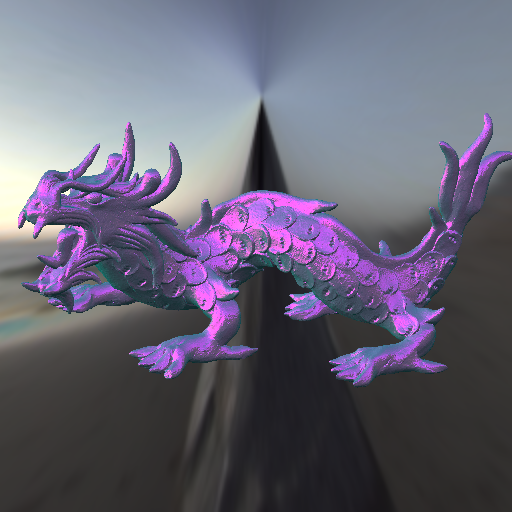
\includegraphics[width=\linewidth]{./Imagens/brdfs/blinn-phong-dragon.png}
    % \legend{ \small (b) Dragão de Stanford}
\endminipage\hfill
\minipage{0.32\textwidth}%
  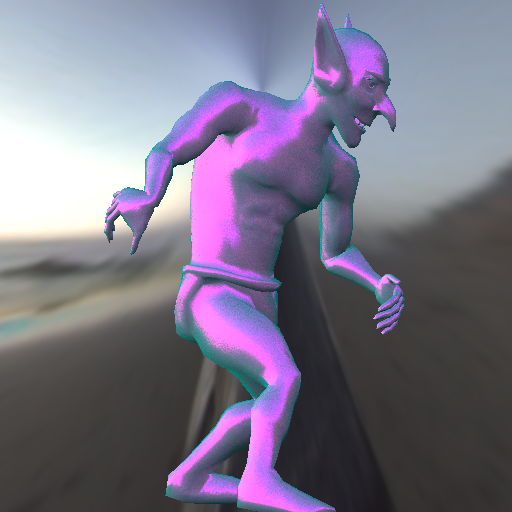
\includegraphics[width=\linewidth]{./Imagens/brdfs/blinn-phong-goblin.png}
    % \legend{ \small (c) Goblin}
\endminipage
\end{figure}
\end{frame}

%%%%%%%%%%%%%%%%%%%%%%%%%%%%%%%%%%%%%%%%%%%%%%%%%
% \subsection{Experimento Blinn-Phong}
%%%%%%%%%%%%%%%%%%%%%%%%%%%%%%%%%%%%%%%%%%%%%%%%%


%%%%%%%%%%%%%%%%%%%%%%%%%%%%%%%%%%%%%%%%%%%%%%%%%
% \subsection{Experimento Cook-Torrance}
%%%%%%%%%%%%%%%%%%%%%%%%%%%%%%%%%%%%%%%%%%%%%%%%%

\begin{frame}
\begin{figure}
    \frametitle{Experimento Cook-Torrance: Equações da BRDF em documento \LaTeX{}}
    \begin{center}
        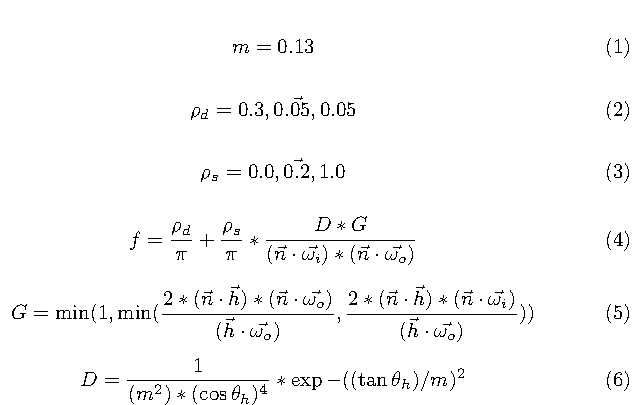
\includegraphics[scale=0.62]{./Imagens/brdfs/cook-torrance.pdf}
    \end{center}
\end{figure}
\end{frame}

%%%%%%%%%%%%%%%%%%%%%%%%%%%%%%%%%%%%%%%%%%%%%%%%%
\begin{frame}[fragile]
    \frametitle{Experimento Cook-Torrance: Código fonte \LaTeX{} da BRDF}
%%%%%%%%%%%%%%%%%%%%%%%%%%%%%%%%%%%%%%%%%%%%%%%%%
    \hspace{1cm}
\begin{lstlisting}[basicstyle=\ttfamily\scriptsize,language=tex, frame=none, inputencoding=utf8]
\begin{equation}
m = 0.13
\end{equation}

\begin{equation}
    \rho_{d} = \vec{0.3,0.05,0.05}
\end{equation}

\begin{equation}
    \rho_{s} = \vec{0.0,0.2,1.0}
\end{equation}

\begin{equation}
f = \frac{\rho_{d}}{\pi} + \frac{\rho_{s}}{\pi} *
\frac{D*G}{({\vec{n}}\cdot{\vec{\omega_{i}}}) *
({\vec{n}}\cdot{\vec{\omega_{o}}})}
\end{equation}

\begin{equation}
G = \min(1,\min( \frac{2 * ({\vec{n}}\cdot{\vec{h}}) * ({\vec{n}}\cdot{\vec{\omega_{o}}}) }
    {({\vec{h}}\cdot{\vec{\omega_{o}}})}, \frac{2 * ({\vec{n}}\cdot{\vec{h}}) *
({\vec{n}}\cdot{\vec{\omega_{i}}}) } {({\vec{h}}\cdot{\vec{\omega_{o}}})}))
\end{equation}

\begin{equation}
D = \frac{1} {(m^{2}) * (\cos{\theta_{h}})^{4}} * \exp{-((\tan{\theta_{h}})/m)^{2}}
\end{equation}
\end{lstlisting}
\end{frame}

\begin{frame}[fragile]
    \frametitle{Experimento Cook-Torrance: Código GLSL da BRDF deste experimento (1 de 2)}
\begin{clang}
analytic ::begin parameters
#[type][name][min val][max val][default val]
::end parameters
::begin shader
//////////// START OF BUILTINS DECLARTION ////////////
vec3 var_0_vec_h;
vec3 var_3_vec_n;
float var_10_theta_h;
float var_11_theta_d;
float var_1_pi;
float var_2_epsilon;
vec3 var_4_vec_omega_i;
float var_5_theta_i;
float var_6_phi_i;
vec3 var_7_vec_omega_o;
float var_8_theta_o;
float var_9_phi_o;
//////////// END OF BUILTINS DECLARTION ////////////
//////////// START OF USER DECLARED ////////////
float var_12_G;
vec3 var_13_rho_s;
float var_14_m;
float var_15_D;
vec3 var_16_rho_d;
vec3 var_17_f;
//////////// END OF USER DECLARED ////////////
//////////// START FUNCTIONS DECLARATIONS ////////////
//////////// END FUNCTIONS DECLARATIONS ////////////
\end{clang}
\end{frame}

\begin{frame}[fragile]
    \frametitle{Experimento Cook-Torrance: Código GLSL da BRDF deste experimento (2 de 2)}
\begin{clang}
vec3 BRDF(vec3 L, vec3 V, vec3 N, vec3 X, vec3 Y) {

  //////////// START OF BUILTINS INITIALIZATION ////////////
  var_0_vec_h = normalize(L + V);
  var_3_vec_n = normalize(N);
  var_1_pi = 3.141592653589793;
  var_2_epsilon = 1.192092896e-07;
  var_4_vec_omega_i = L;
  var_5_theta_i = atan(var_4_vec_omega_i.y, var_4_vec_omega_i.x);
  var_6_phi_i = atan(sqrt(var_4_vec_omega_i.y * var_4_vec_omega_i.y +
                          var_4_vec_omega_i.x * var_4_vec_omega_i.x), var_4_vec_omega_i.z);
  var_7_vec_omega_o = V;
  var_8_theta_o = atan(var_7_vec_omega_o.y, var_7_vec_omega_o.x);
  var_9_phi_o = atan(sqrt(var_7_vec_omega_o.y * var_7_vec_omega_o.y + var_7_vec_omega_o.x * var_7_vec_omega_o.x),
                     var_7_vec_omega_o.z);
  var_10_theta_h = acos(dot(var_0_vec_h, N));
  var_11_theta_d = acos(dot(var_0_vec_h, var_4_vec_omega_i));
  //////////// END OF BUILTINS INITIALIZATION ////////////

  var_12_G = min(1.0, min((((2.0 * (dot(var_3_vec_n, var_0_vec_h))) * (dot(var_3_vec_n, var_7_vec_omega_o))) / (dot(var_0_vec_h, var_7_vec_omega_o))), (((2.0 * (dot(var_3_vec_n, var_0_vec_h))) *
                            (dot(var_3_vec_n, var_4_vec_omega_i))) /
                           (dot(var_0_vec_h, var_7_vec_omega_o)))));
  var_13_rho_s = vec3(0.0, 0.2, 1.0);
  var_14_m = 0.13;
  var_15_D = ((1.0 / ((pow(var_14_m, 2.0)) * pow((cos(var_10_theta_h)), 4.0))) *
              exp((-pow((((tan(var_10_theta_h)) / var_14_m)), 2.0))));
  var_16_rho_d = vec3(0.3, 0.05, 0.05);
  var_17_f = ((var_16_rho_d / var_1_pi) + ((var_13_rho_s / var_1_pi) * ((var_15_D * var_12_G) / ((dot(var_3_vec_n, var_4_vec_omega_i)) * (dot(var_3_vec_n, var_7_vec_omega_o))))));
  return vec3(var_17_f);
}
\end{clang}
\end{frame}

\begin{frame}{Experimento Cook-Torrance: Plots de Distruição de Reflexão}
\begin{figure}[H]
  
\caption{\small{\textit{Plots} da distribuição de reflexão especular e difusa do experimento cook-torrance.}}
    \label{fig-cook-torrance-plots}
\minipage{0.48\textwidth}
    \vspace{42px}
  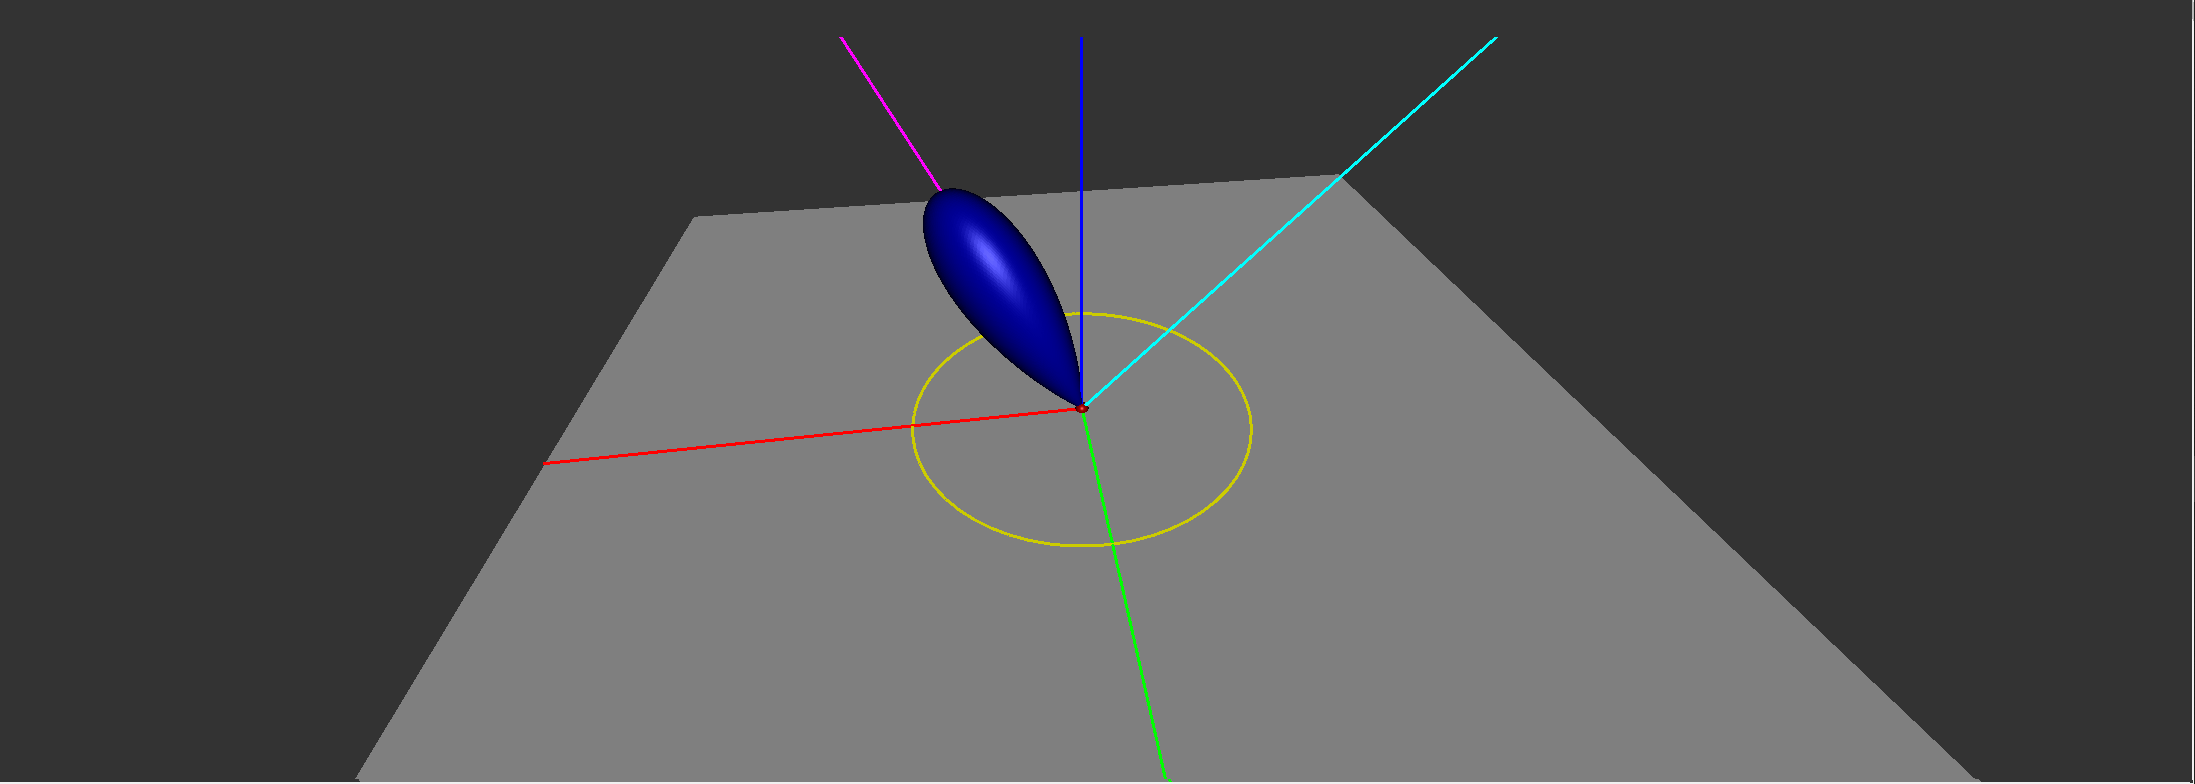
\includegraphics[width=\linewidth]{./Imagens/brdfs/cook-torrance-3D-plot}
    % \caption{\small{(a)}}\label{fig:awesome_image1}
    % \vspace{0.1px}
    % \legend{ \small (a) 3D \textit{plot}}
\endminipage\hfill
\minipage{0.48\textwidth}
  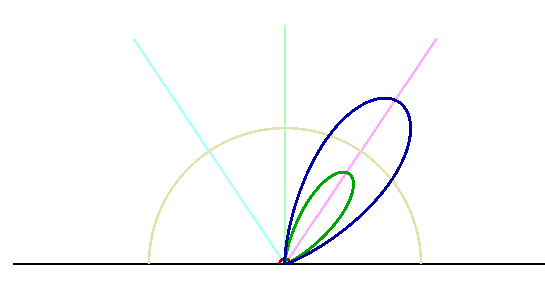
\includegraphics[width=\linewidth]{./Imagens/brdfs/cook-torrance-polar-plot-log.png}
    % \legend{ \small (b) \textit{Polar plot}}
    % \caption{\small{(b)}}\label{fig:awesome_image1}
\endminipage\hfill
\end{figure}
\end{frame}

\begin{frame}{Experimento Cook-Torrance: Objetos 3D renderizados para esta BRDF}
\begin{figure}[H]
    \label{fig-cook-torrance-eqlang}
\minipage{0.32\textwidth}
  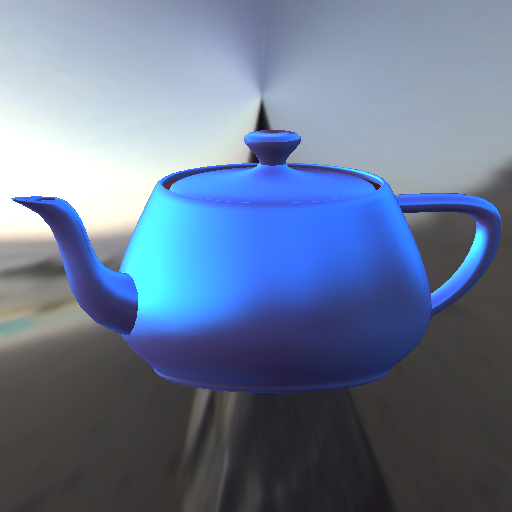
\includegraphics[width=\linewidth]{./Imagens/brdfs/cook-torrance-teapot.png}
    % \legend{ \small (a) \textit{Teapot}}
\endminipage\hfill
\minipage{0.32\textwidth}
  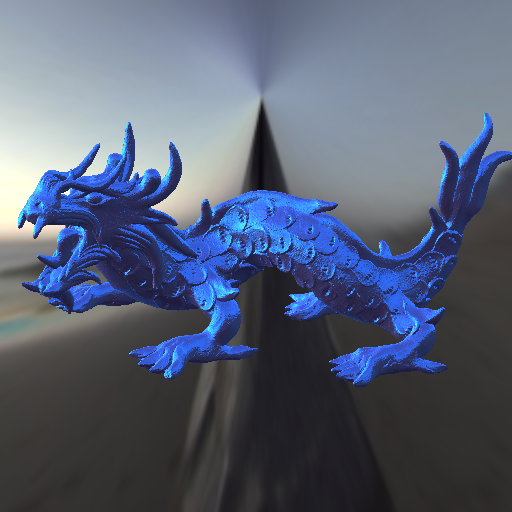
\includegraphics[width=\linewidth]{./Imagens/brdfs/cook-torrance-dragon.png}
    % \legend{ \small (b) Dragão de Stanford}
\endminipage\hfill
\minipage{0.32\textwidth}%
  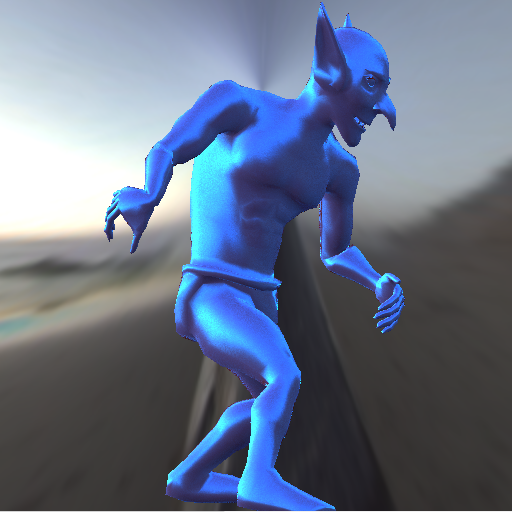
\includegraphics[width=\linewidth]{./Imagens/brdfs/cook-torrance-goblin.png}
    % \legend{ \small (c) Goblin}
\endminipage
\end{figure}
\end{frame}

%%%%%%%%%%%%%%%%%%%%%%%%%%%%%%%%%%%%%%%%%%%%%%%%%
% \subsection{Experimento Cook-Torrance}
%%%%%%%%%%%%%%%%%%%%%%%%%%%%%%%%%%%%%%%%%%%%%%%%%


%%%%%%%%%%%%%%%%%%%%%%%%%%%%%%%%%%%%%%%%%%%%%%%%%
% \subsection{Experimento Edwards-2006}
%%%%%%%%%%%%%%%%%%%%%%%%%%%%%%%%%%%%%%%%%%%%%%%%%

\begin{frame}
\begin{figure}
    \frametitle{Experimento Edwards-2006: Equações da BRDF em documento \LaTeX{}}
    \footnote{\tiny{Experimento adicionado aos slides para demonstrar definição de funções no formato $f(x,y) = x+y$.}}
    \begin{center}
        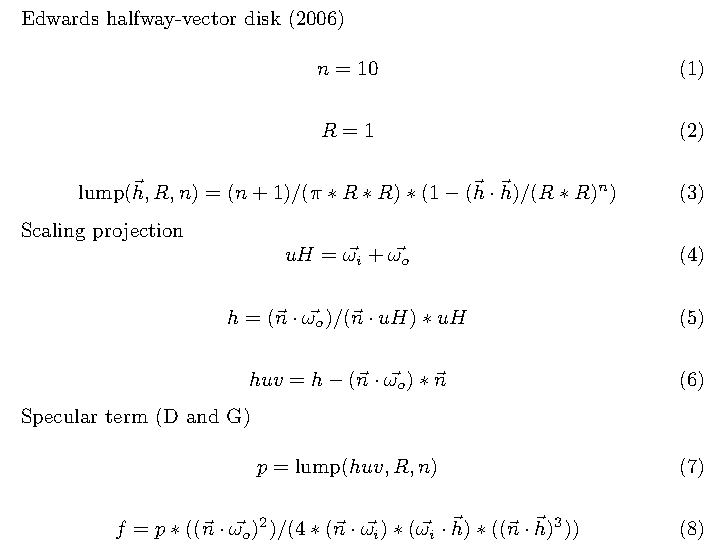
\includegraphics[scale=0.52]{./Imagens/brdfs/edwards-2006.pdf}
    \end{center}
\end{figure}
\end{frame}

%%%%%%%%%%%%%%%%%%%%%%%%%%%%%%%%%%%%%%%%%%%%%%%%%
\begin{frame}[fragile]
    \frametitle{Experimento Edwards-2006: Código fonte \LaTeX{} da BRDF}
%%%%%%%%%%%%%%%%%%%%%%%%%%%%%%%%%%%%%%%%%%%%%%%%%
    \vspace{-0.3cm}
    \hspace{2cm}
\begin{lstlisting}[basicstyle=\ttfamily\scriptsize,language=tex, frame=none, inputencoding=utf8]
\begin{equation}
n = 10
\end{equation}
\begin{equation}
R = 1
\end{equation}

\begin{equation}
\text{lump}(\vec{h}, R, n) = (n+1)/(\pi*R*R) * (1-(\vec{h} \cdot \vec{h})/(R*R)^ n)
\end{equation}

Scaling projection
\begin{equation}
    uH = \vec{\omega_i}+\vec{\omega_o} % // unnormalized H
\end{equation}
\begin{equation}
    h = (\vec{n} \cdot \vec{\omega_o}) / (\vec{n} \cdot uH) * uH
\end{equation}
\begin{equation}
    huv = h - (\vec{n} \cdot \vec{\omega_o}) * \vec{n}
\end{equation}
Specular term (D and G)
\begin{equation}
    p = \text{lump}(huv, R, n)
\end{equation}
\begin{equation}
    f = p * ((\vec{n} \cdot \vec{\omega_o})^ 2)
    / (4 * (\vec{n} \cdot \vec{\omega_i})
    * (\vec{\omega_i} \cdot \vec{h}) * ((\vec{n} \cdot \vec{h})^ 3))
\end{equation}
\end{lstlisting}
\end{frame}

\begin{frame}[fragile]
    \frametitle{Experimento Edwards-2006: Código GLSL da BRDF deste experimento (1 de 2)}
\begin{clang}
analytic ::begin parameters
#[type][name][min val][max val][default val]
::end parameters
::begin shader
//////////// START OF BUILTINS DECLARTION ////////////
vec3 var_0_vec_h;
vec3 var_3_vec_n;
float var_10_theta_h;
float var_11_theta_d;
float var_1_pi;
float var_2_epsilon;
vec3 var_4_vec_omega_i;
float var_5_theta_i;
float var_6_phi_i;
vec3 var_7_vec_omega_o;
float var_8_theta_o;
float var_9_phi_o;
//////////// END OF BUILTINS DECLARTION ////////////
//////////// START OF USER DECLARED ////////////
vec3 var_15_uH;
vec3 var_16_h;
float var_14_n;
vec3 var_17_huv;
float var_13_R;
float var_18_p;
float var_19_f;
//////////// END OF USER DECLARED ////////////
//////////// START FUNCTIONS DECLARATIONS ////////////
float var_12_text_lump(vec3 var_0_vec_h, float var_13_R, float var_14_n) {
  return ((((var_14_n + 1.0)) / (((var_1_pi * var_13_R) * var_13_R))) *
          ((1.0 - ((dot(var_0_vec_h, var_0_vec_h)) /
                   pow(((var_13_R * var_13_R)), var_14_n)))));
}
\end{clang}
\end{frame}

\begin{frame}[fragile]
    \frametitle{Experimento Edwards-2006: Código GLSL da BRDF deste experimento (2 de 2)}
\begin{clang}
//////////// END FUNCTIONS DECLARATIONS ////////////
vec3 BRDF(vec3 L, vec3 V, vec3 N, vec3 X, vec3 Y) {
  //////////// START OF BUILTINS INITIALIZATION ////////////
  var_0_vec_h = normalize(L + V);
  var_3_vec_n = normalize(N);
  var_1_pi = 3.141592653589793;
  var_2_epsilon = 1.192092896e-07;
  var_4_vec_omega_i = L;
  var_5_theta_i = atan(var_4_vec_omega_i.y, var_4_vec_omega_i.x);
  var_6_phi_i = atan(sqrt(var_4_vec_omega_i.y * var_4_vec_omega_i.y +
                          var_4_vec_omega_i.x * var_4_vec_omega_i.x), var_4_vec_omega_i.z);
  var_7_vec_omega_o = V;
  var_8_theta_o = atan(var_7_vec_omega_o.y, var_7_vec_omega_o.x);
  var_9_phi_o = atan(sqrt(var_7_vec_omega_o.y * var_7_vec_omega_o.y +
                          var_7_vec_omega_o.x * var_7_vec_omega_o.x), var_7_vec_omega_o.z);
  var_10_theta_h = acos(dot(var_0_vec_h, N));
  var_11_theta_d = acos(dot(var_0_vec_h, var_4_vec_omega_i));
  //////////// END OF BUILTINS INITIALIZATION ////////////
  var_15_uH = (var_4_vec_omega_i + var_7_vec_omega_o);
  var_16_h = (((dot(var_3_vec_n, var_7_vec_omega_o)) /
    (dot(var_3_vec_n, var_15_uH))) * var_15_uH);
  var_14_n = 10.0;
  var_17_huv = (var_16_h - ((dot(var_3_vec_n, var_7_vec_omega_o)) * var_3_vec_n));
  var_13_R = 1.0;
  var_18_p = var_12_text_lump(var_17_huv, var_13_R, var_14_n);
  var_19_f = ((var_18_p * (pow((dot(var_3_vec_n, var_7_vec_omega_o)), 2.0))) /
              ((((4.0 * (dot(var_3_vec_n, var_4_vec_omega_i))) *
                 (dot(var_4_vec_omega_i, var_0_vec_h))) * (pow((dot(var_3_vec_n, var_0_vec_h)), 3.0)))));
  return vec3(var_19_f);
}
\end{clang}
\end{frame}

\begin{frame}{Experimento Edwards-2006: Plots de Distruição de Reflexão}
\begin{figure}[H]
  
\caption{\small{\textit{Plots} da distribuição de reflexão especular e difusa do experimento edwards-2006.}}
    \label{fig-edwards-2006-plots}
\minipage{0.48\textwidth}
    \vspace{42px}
  
\includegraphics[width=\linewidth]{./Imagens/brdfs/edwards-2006-3D-plot}
    % \caption{\small{(a)}}\label{fig:awesome_image1}
    % \vspace{0.1px}
    % \legend{ \small (a) 3D \textit{plot}}
\endminipage\hfill
\minipage{0.48\textwidth}
  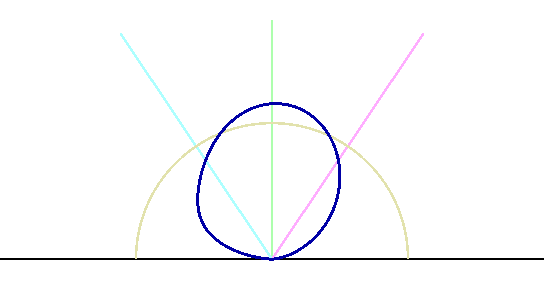
\includegraphics[width=\linewidth]{./Imagens/brdfs/edwards-2006-polar-plot.png}
    % \legend{ \small (b) \textit{Polar plot}}
    % \caption{\small{(b)}}\label{fig:awesome_image1}
\endminipage\hfill
\end{figure}
\end{frame}

\begin{frame}{Experimento Edwards-2006: Objetos 3D renderizados para esta BRDF}
\begin{figure}[H]
    \label{fig-edwards-2006-eqlang}
\minipage{0.32\textwidth}
  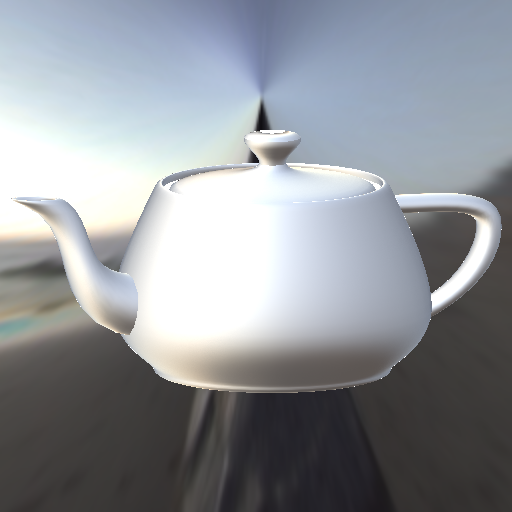
\includegraphics[width=\linewidth]{./Imagens/brdfs/edwards-2006-teapot.png}
    % \legend{ \small (a) \textit{Teapot}}
\endminipage\hfill
\minipage{0.32\textwidth}
  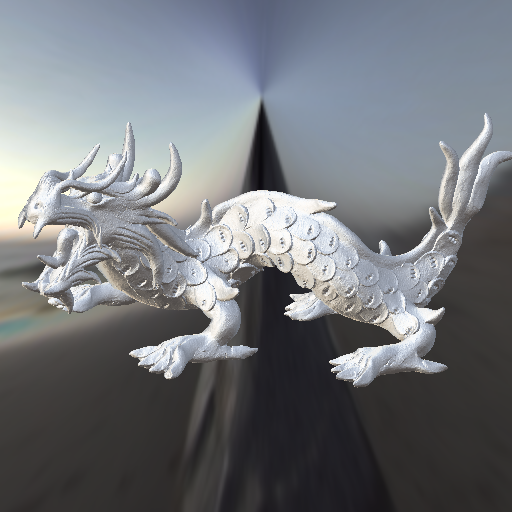
\includegraphics[width=\linewidth]{./Imagens/brdfs/edwards-2006-dragon.png}
    % \legend{ \small (b) Dragão de Stanford}
\endminipage\hfill
\minipage{0.32\textwidth}%
  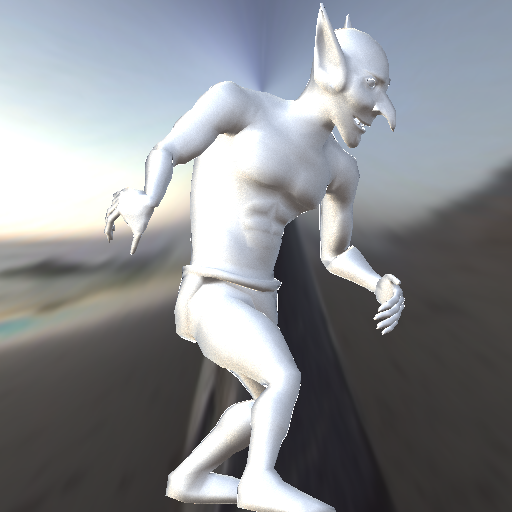
\includegraphics[width=\linewidth]{./Imagens/brdfs/edwards-2006-goblin.png}
    % \legend{ \small (c) Goblin}
\endminipage
\end{figure}
\end{frame}

%%%%%%%%%%%%%%%%%%%%%%%%%%%%%%%%%%%%%%%%%%%%%%%%%
% \subsection{Experimento Edwards-2006}
%%%%%%%%%%%%%%%%%%%%%%%%%%%%%%%%%%%%%%%%%%%%%%%%%


\begin{frame}[fragile]{Resultados: Visão Simplificada dos Outros Experimentos}
   \begin{table}
       \centering
       \scriptsize % Tamanho de texto ajustável (\scriptsize ou \footnotesize)
       \begin{tabular}{|c|c|c|c|c|}
           \hline
           \textbf{Experimento}        & Blinn-Phong     & Cook-Torrance   & Ward           & Ashikhmin-Shirley \\ \hline
           \textbf{Visualização} &
           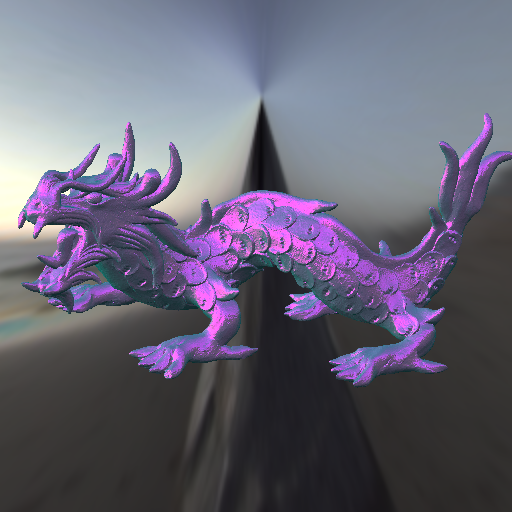
\includegraphics[scale=0.14]{./Imagens/brdfs/blinn-phong-dragon.png} & 
           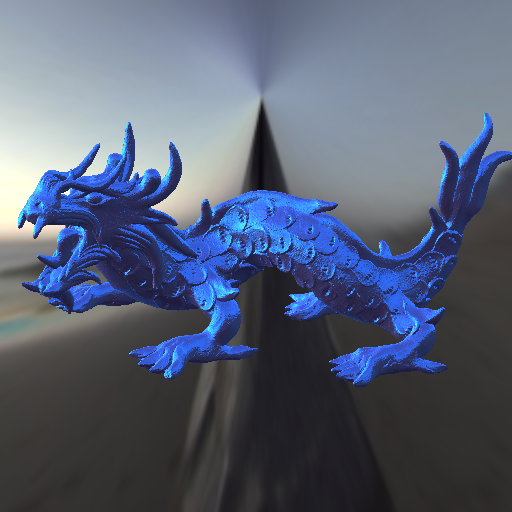
\includegraphics[scale=0.14]{./Imagens/brdfs/cook-torrance-dragon.png} & 
           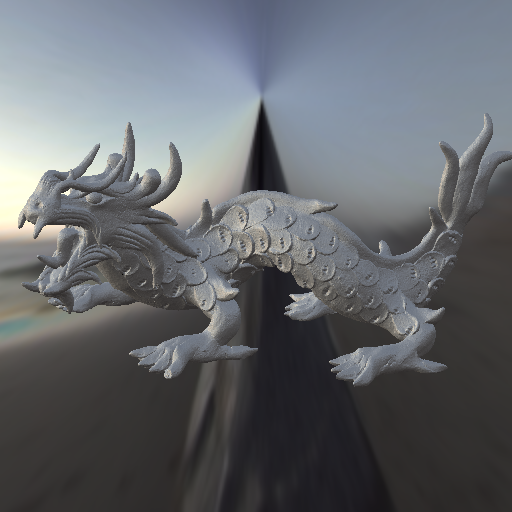
\includegraphics[scale=0.14]{./Imagens/brdfs/ward-dragon.png} & 
           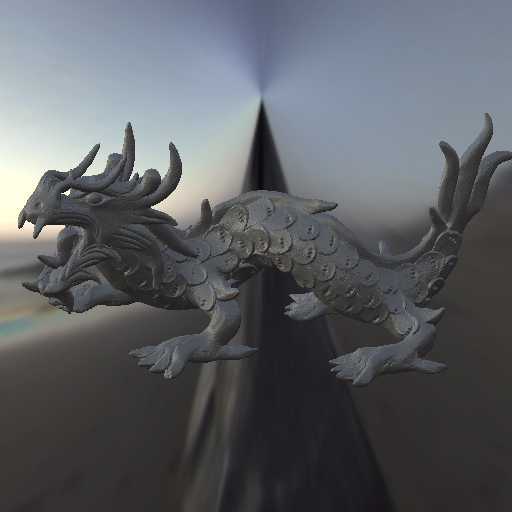
\includegraphics[scale=0.14]{./Imagens/brdfs/ashikhmin-shirley-close-to-original-dragon.png} \\ \hline
       \end{tabular}
   \end{table}

   \begin{table}
       \centering
       \scriptsize % Tamanho de texto ajustável (\scriptsize ou \footnotesize)
       \begin{tabular}{|c|c|c|c|c|}
           \hline
           \textbf{Experimento}        & Oren-Nayar     & Ashikhmin-Shirley$_2$   & Cook-Torrance$_2$ & Dür \\ \hline
           \textbf{Visualização} &
           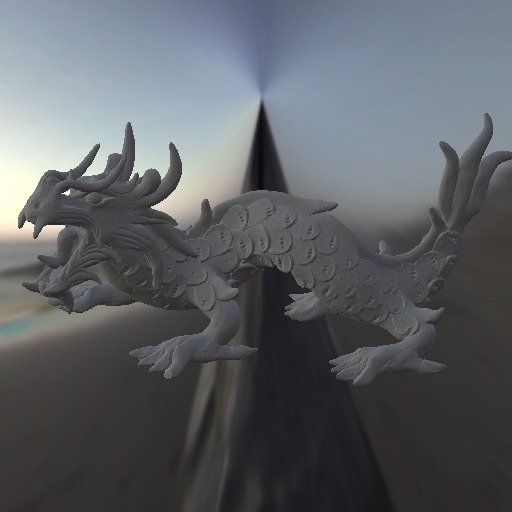
\includegraphics[scale=0.14]{./Imagens/brdfs/oren-nayar-dragon.png} &
           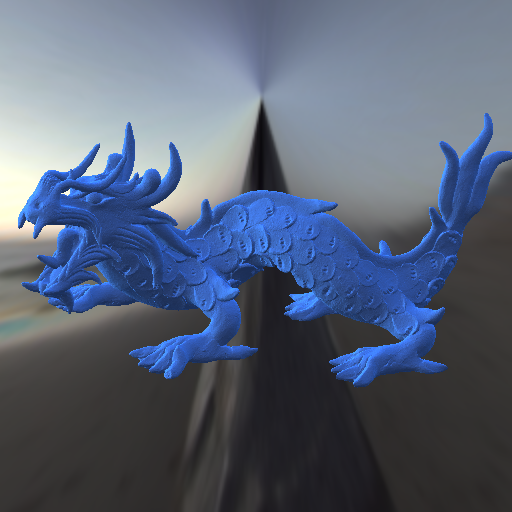
\includegraphics[scale=0.14]{./Imagens/brdfs/ashikhmin-shirley-alternative-dragon.png} &
           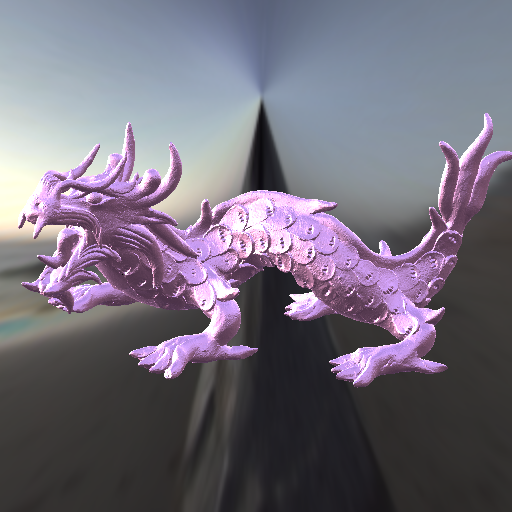
\includegraphics[scale=0.14]{./Imagens/brdfs/cook-torrance-alternative-dragon.png} &
           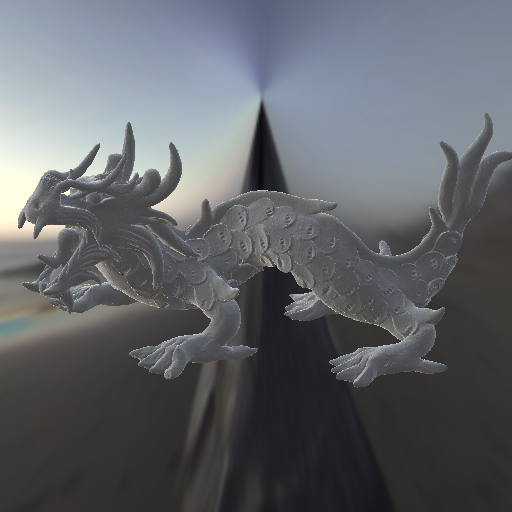
\includegraphics[scale=0.14]{./Imagens/brdfs/duer-dragon.png} \\ \hline
       \end{tabular}
   \end{table}

   \begin{table}
       \centering
       \scriptsize % Tamanho de texto ajustável (\scriptsize ou \footnotesize)
       \begin{tabular}{|c|c|c|c|}
           \hline
           \textbf{Experimento}        & Edwards-2006     & Kajiya-Kay-1989$_*$   & Minnaert \\ \hline
           \textbf{Visualização} &
           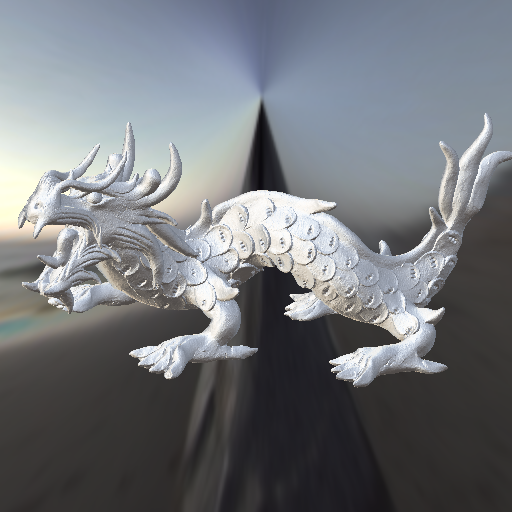
\includegraphics[scale=0.14]{./Imagens/brdfs/edwards-2006-dragon.png} &
           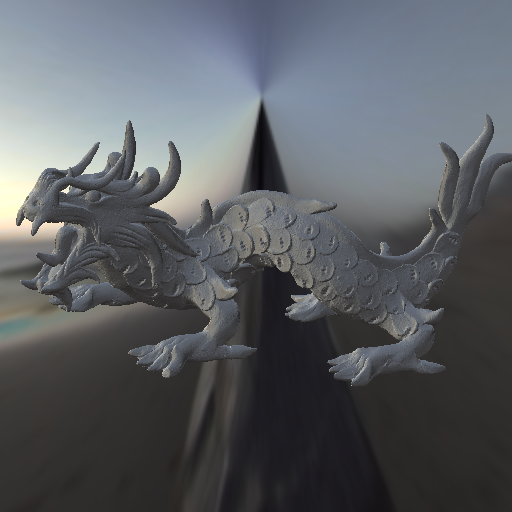
\includegraphics[scale=0.14]{./Imagens/brdfs/aniso-dragon.png} &
           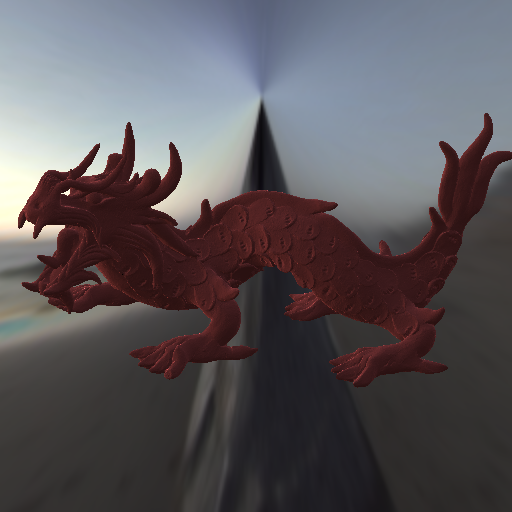
\includegraphics[scale=0.14]{./Imagens/brdfs/minnaert-dragon.png}\\ \hline
       \end{tabular}
   \end{table}
\end{frame}


\include{Content/Slides/sections/Conclusões.tex}




\begin{frame}{Referências}
    % \cite{*}
    \printbibliography[heading=none]
    % \printbibliography
    % \bibliography{Bibliografia}
\end{frame}

\begin{frame}{Modelos de BRDFs}
    \begin{itemize}
        \item BRDF (Bidirectional Reflectance Distribution Function):  
              Função que descreve como a luz é refletida por uma superfície.
        \item Apresentaremos modelos clássicos de BRDFs:
        \begin{itemize}
            \item BRDF Pura Especular.
            \item BRDF Difusa Ideal.
            \item BRDF Brilhante.
            \item BRDF Retro-Refletora.
        \end{itemize}
    \end{itemize}
\end{frame}

% BRDF Pura Especular
\begin{frame}{BRDF Pura Especular}
    \begin{itemize}
        \item Superfície reflete luz apenas em uma direção.
        \item Segue a Lei da Reflexão:
        \[
        f(\omega_i, \omega_o) = k_s \cdot \delta(\omega_i - \omega_o)
        \]
        \item Materiais típicos: metal polido, vidro.
    \end{itemize}
    \begin{figure}[H]
        \centering
        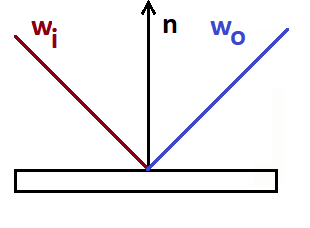
\includegraphics[scale=0.5]{./Imagens/specular-2d.png}
        \caption{\small Reflexão especular. Raio incidente em vermelho e raio refletido em azul.}
    \end{figure}
\end{frame}

% BRDF Difusa Ideal
\begin{frame}{BRDF Difusa Ideal}
    \begin{itemize}
        \item Reflexão uniforme em todas as direções.
        \item Função BRDF:
        \[
        f(\omega_i, \omega_o) = \frac{\rho_d}{\pi} \cdot \cos \theta
        \]
        \item Exemplos: tinta fosca, papel.
    \end{itemize}
    \begin{figure}[H]
        \centering
        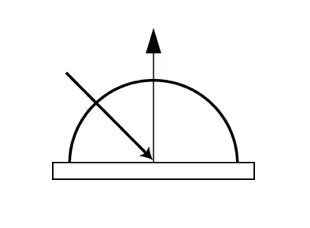
\includegraphics[scale=0.5]{./Imagens/diffuse-2d.png}
        \caption{\small Reflexão difusa. Raios refletidos independem do ângulo de entrada.}
    \end{figure}
\end{frame}

% BRDF Brilhante
\begin{frame}{BRDF Brilhante}
    \begin{itemize}
        \item Combina reflexões especulares e difusas.
        \item Modelo típico: Blinn-Phong.
    \end{itemize}
    \begin{figure}[H]
        \centering
        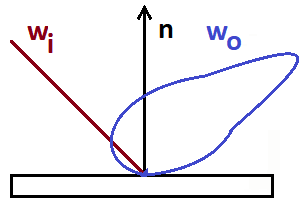
\includegraphics[scale=0.5]{./Imagens/glossy-2d.png}
        \caption{\small Reflexão \textit{glossy}.}
    \end{figure}
\end{frame}

% BRDF Retro-Refletora
\begin{frame}{BRDF Retro-Refletora}
    \begin{itemize}
        \item Redireciona a luz de volta à fonte.
        \item Utilizado em superfícies como placas de trânsito e sinais de segurança.
    \end{itemize}
    \begin{figure}[H]
        \centering
        \includegraphics[scale=0.5]{./Imagens/retro-reflection-2d.png}
        \caption{\small Reflexão retro-refletora.}
    \end{figure}
\end{frame}

\begin{frame}{BRDF: Função de Refletância Bidirecional}
    \begin{itemize}
        \item BRDF (\( f \)) descreve como a luz reflete em diferentes direções:
        \[
        f(\omega_i, \omega_o) = \frac{dL_o(\omega_o)}{L_i(\omega_i) \cos(\theta_i) d\omega_i}
        \]
        \item Propriedades:
        \begin{enumerate}
            \item Positividade: \( f \geq 0 \).  
            \item Conservação de energia: \(\int_{\Omega} f \cos(\theta_i) d\omega_i \leq 1\).
            \item Reciprocidade de Helmholtz: \( f(\omega_i, \omega_o) = f(\omega_o, \omega_i) \).
        \end{enumerate}
    \end{itemize}
\end{frame}

\begin{frame}{Radiometria: Introdução}
    \begin{itemize}
        \item Estuda a interação da luz com superfícies na computação gráfica.
        \item Quantifica energia luminosa:
        \begin{itemize}
            \item Brilho da fonte de luz.
            \item Iluminação e refletância da superfície.
        \end{itemize}
        \item Fundamenta a renderização realista de cenas tridimensionais.
    \end{itemize}
\end{frame}

\begin{frame}{Energia Radiante $Q$}
    \begin{itemize}
        \item Quantifica a energia total dos fótons atingindo uma superfície.
        \item Fórmula:
        \[
            Q = \frac{hc}{\lambda}
        \]

        onde:
        \begin{itemize}
            \item \( h \): Constante de Planck.  
            \item \( c \): Velocidade da luz.  
            \item \( \lambda \): Comprimento de onda.  
        \end{itemize}
    \end{itemize}
\end{frame}

\begin{frame}{Fluxo Radiante e Irradiância}
    \begin{itemize}
        \item Fluxo Radiante: Energia por unidade de tempo (\( J/s \)):
        \[
            \phi = \frac{dQ}{dt} % \left[\text{J/s}\right]
        \]
        \item Irradiância: Fluxo radiante por unidade de área:
        \[
        E(p) = \frac{d\phi(p)}{dA} %  \left[ \frac{\text{J}} {s\cdot m^2} \right]
        \]
    \item Quantifica os impactos de fótons em uma superfície.\footnote{\footnotesize{Saber quantos fótons "tocam" uma superfície por segundo, é saber quão iluminado é aquela parte do objeto.}}
    \end{itemize}
\end{frame}

\begin{frame}{Radiância}
    Radiância (\( L \)): Fluxo radiante por unidade de área e ângulo sólido:
    \[
    L = \frac{d^2\Phi}{dA \, d\omega \cos(\theta)}
    \]
    Onde:
    \begin{itemize}
        \item \( d\omega \): Ângulo sólido (em sr).  
        \item \( \theta \): Ângulo entre direção de incidência e normal da superfície.
    \end{itemize}
\end{frame}



\begin{frame}{Visualização da Radiância}
    \begin{itemize}
        \item Radiância considera direção específica no hemisfério sobre a superfície.
    \end{itemize}

\begin{figure}[h]
        \caption{\label{radiance-img} \small Visualização da radiância em uma direção específica do hemisfério. }
            \includegraphics[scale=0.5]{./Imagens/irradiance_hemisphere.png}
  % \legend{ \small Fonte: \cite{pbr}. Adaptada.}
\end{figure}


\begin{figure}[h]
  \caption{\label{solid-angle} \small   Ângulo sólido s do objeto B visto pelo ponto p. }
            \includegraphics[scale=0.5]{./Imagens/solid_angle.png}
  % \legend{ \small Fonte: \cite{pbr}.}
\end{figure}
\end{frame}

\begin{frame}{Árvore SVG}
\end{frame}



\end{document}



